\documentclass[utf8]{frontiersSCNS} % for Science, Engineering and Humanities and Social Sciences articles
%\documentclass[utf8]{frontiersHLTH} % for Health articles
%\documentclass[utf8]{frontiersFPHY} % for Physics and Applied Mathematics and Statistics articles
%\setcitestyle{square} % for Physics and Applied Mathematics and Statistics articles
\usepackage[french]{babel}
\usepackage{url,hyperref,lineno,microtype,subcaption}
\usepackage[onehalfspacing]{setspace}
\usepackage[toc,page]{appendix} 
\usepackage{pdfpages}
\usepackage{color, colortbl}
\usepackage{multirow}
\linenumbers


% Leave a blank line between paragraphs instead of using \\


\def\keyFont{\fontsize{8}{11}\helveticabold }
\def\firstAuthorLast{Dermy {et~al.}} %use et al only if is more than 1 author
\def\Authors{Oriane Dermy\,$^{1,*}$, Alexandros Paraschos\,$^{2,4}$, Marco Ewerton\,$^{2}$,  Jan Peters\,$^{2,3}$, Fran\c cois Charpillet\,$^{1}$ and Serena Ivaldi\,$^{1}$}
% Affiliations should be keyed to the author's name wifth superscript numbers and be listed as follows: Laboratory, Institute, Department, Organisation, City, State abbreviation (USA, Canada, Australia), and Country (without detailed address information such as city zip codes or street names).
% If one of the authors has a change of address, list the new address below the correspondence details using a superscript symbol and use the same symbol to indicate the author in the author list.
\def\Address{$^{1}$ Inria, Villers-lés-Nancy, 54600, France; \\Université de Lorraine, Loria, UMR7503, Vandoeuvre, 54500, France; \\
CNRS, Loria, UMR7503, Vandoeuvre, 54500, France \\
        {\tt\small name.surname@inria.fr}\\
$^{2}$TU Darmstadt, Darmstadt, Germany\\
$^{3}$Max Planck Institute for Intelligent Systems, Tubingen, Germany\\
$^{4}$Data Lab, Volkswagen Group, 80805 Munich, Germany}
% The Corresponding Author should be marked with an asterisk
% Provide the exact contact address (this time including street name and city zip code) and email of the corresponding author
\def\corrAuthor{Corresponding Author}

\def\corrEmail{oriane.dermy@inria.fr}


%%%% PACKAGES %%%%
%
%% The following packages can be found on http:\\www.ctan.org
%\usepackage{graphics} % for pdf, bitmapped graphics files
%%\usepackage{epsfig} % for postscript graphics files
%%\usepackage{mathptmx} % assumes new font selection scheme installed
%%\usepackage{times} % assumes new font selection scheme installed
%%\usepackage{amsmath} % assumes amsmath package installed
%%\usepackage{amssymb}  % assumes amsmath package installed
%
%% *** MATH PACKAGES ***
%%
%\usepackage{amsmath}
%% A popular package from the American Mathematical Society that provides
%% many useful and powerful commands for dealing with mathematics.
%%
%% Note that the amsmath package sets \interdisplaylinepenalty to 10000
%% thus preventing page breaks from occurring within multiline equations. Use:
%%\interdisplaylinepenalty=2500
%% after loading amsmath to restore such page breaks as IEEEtran.cls normally
%% does. amsmath.sty is already installed on most LaTeX systems. The latest
%% version and documentation can be obtained at:
%% http://www.ctan.org/pkg/amsmath
%\usepackage{amssymb}  % assumes amsmath package installed
%\usepackage{bm} 
\usepackage{dsfont}

%\usepackage{bbm}
%\usepackage{bbold}
%
%% *** SPECIALIZED LIST PACKAGES ***
%%
%%\usepackage{algorithmic}
%% algorithmic.sty was written by Peter Williams and Rogerio Brito.
%% This package provides an algorithmic environment fo describing algorithms.
%% You can use the algorithmic environment in-text or within a figure
%% environment to provide for a floating algorithm. Do NOT use the algorithm
%% floating environment provided by algorithm.sty (by the same authors) or
%% algorithm2e.sty (by Christophe Fiorio) as the IEEE does not use dedicated
%% algorithm float types and packages that provide these will not provide
%% correct IEEE style captions. The latest version and documentation of
%% algorithmic.sty can be obtained at:
%% http://www.ctan.org/pkg/algorithms
%% Also of interest may be the (relatively newer and more customizable)
%% algorithmicx.sty package by Szasz Janos:
%% http://www.ctan.org/pkg/algorithmicx
%\usepackage{algorithm}
%\usepackage{algpseudocode}
%\usepackage{tcolorbox}
%\usepackage{tikz}
%
%% *** PDF, URL AND HYPERLINK PACKAGES ***
%%
%\usepackage{url}
%% url.sty was written by Donald Arseneau. It provides better support for
%% handling and breaking URLs. url.sty is already installed on most LaTeX
%% systems. The latest version and documentation can be obtained at:
%% http://www.ctan.org/pkg/url
%% Basically, \url{my_url_here}.

% https://fr.mathworks.com/matlabcentral/fileexchange/8015-m-code-latex-package
% load package with some of the available options (default by template)
\usepackage[framed,numbered,autolinebreaks,useliterate]{mcode}
 \usepackage{ulem}

\newcommand{\rev}[1]{\textcolor{blue}{#1}}
\newcommand{\ori}[1]{\textcolor{teal}{#1}}


\newcommand{\toimprove}[1]{\textcolor{teal}{#1}}
\newcommand{\todo}[1]{\textcolor{red}{\textbf{/*#1*/}}}
\newcommand{\quest}[1]{\textcolor{green}{\textit{#1}}}

\newcommand*\rfrac[2]{{}^{#1}\!/_{#2}}

% pick one of these colors
%black, blue, brown, cyan, darkgray, gray, green, lightgray, lime, magenta, olive, orange, pink, purple, red, teal, violet, white, yellow.

\newcommand{\colorcmaes}{teal}
\newcommand{\colorcmaesbackground}{hite}
\newcommand{\colorcmaeschange}{blue}



% ***************************************************
% ***************************************************


\begin{document}


\onecolumn
\firstpage{1}

\title[Prédiction de l'intention lors d'interaction avec le robot iCub]{Prédiction de l'intention lors d'interaction physique avec le robot iCub, à l'aide de primitives de mouvements probabilistes} 

\author[\firstAuthorLast ]{\Authors} %This field will be automatically populated
\address{} %This field will be automatically populated
\correspondance{} %This field will be automatically populated

\extraAuth{}% If there are more than 1 corresponding author, comment this line and uncomment the next one.
%\extraAuth{corresponding Author2 \\ Laboratory X2, Institute X2, Department X2, Organisation X2, Street X2, City X2 , State XX2 (only USA, Canada and Australia), Zip Code2, X2 Country X2, email2@uni2.edu}


\maketitle
%%%%%%%%%%%%%%%%%%%%%%%%%%%%%%%%%%%%%%%%%%%%%%%%%%%%%%%%%%%%%%%%%%%%%%%%%%%%%%%%

%\newpage
%%%%%%%%%%%%%%%%%%%%%%%%%%%%%%%%%%%%%%%%%%%%%%%%%%%%%%%%%%%%%%%%%%%%%%%%%%%%%%%%
\section{Cadre théorique}
\label{sec:theory}

Dans cette section, nous présentons le cadre théorique utilisé afin de répondre au problème de la reconnaissance de l'intention. 

%Pour cela, nous présenterons d'abord dans la Section~\ref{LearningSimpleProMP} le fonctionnement de la méthode \textit{ProMPs}, puis dans la Section~\ref{sec:predict} son utilisation qui consiste à la prédiction de la continuation de trajectoires, à partir de l'observation du commencement de celles-ci.

Pour cela, la Section~\ref{LearningSimpleProMP} formule le problème de l'apprentissage d'une primitive à l'aide de la méthode \textit{ProMP}, pour un exemple jouet. Cet apprentissage de primitive sera effectué à l'aide de plusieurs trajectoires de démonstration. 
Puis, la Section~\ref{sec:predict} formule et fournit la solution au problème de prédiction de la trajectoire \og future \fg{}, à partir des premières observations de celle-ci.
De plus, dans la Section~\ref{sec:predictDuration}, nous discutons du problème de prédiction de la 
%\toimprove{modulation du temps}, c'est-à-dire la prédiction de la 
durée globale de la trajectoire qui a été inférée. Ce problème n'est pas trivial puisque, lors de l'apprentissage des \textit{ProMPs}, les trajectoires de démonstration sont \og normalisées \fg{} par rapport au temps. \footnote{Pour certaines tâches, telles que les tâches consistant à atteindre une cible, il est raisonnable de supposer que la différence de durée des trajectoires est négligeable. Cependant, pour d'autres tâches, la durée des trajectoires peut varier, surtout lorsque celles-ci sont effectuées par des personnes différentes.}
Finalement, la Section~\ref{sec:ManyProMP} présente comment reconnaître, à partir de l'initiation d'une trajectoire, quelle compétence doit être sollicitée parmi les nombreuses apprises (modélisées par des \textit{ProMPs}). En plus de déterminer la compétence sollicitée, cette Section présente comment prédire la continuation de la trajectoire initiée.

Ainsi, ces trois Sections présentent les aspects théoriques de l'utilisation de la méthode \textit{ProMP}, permettant de créer notre application permettant la reconnaissance des intentions.

Ces problèmes théoriques sont ensuite illustrés avec des exemples détaillés.
Ainsi, la Section \ref{sec:example1DOF} explique comment utiliser le logiciel (introduits dans la Section~\ref{sec:softwareOverview}) dans le cas d'apprentissage d'une trajectoire à une dimension.
Puis, les Sections \ref{sec:3ProMPsAppli} et \ref{sec:appliRealIcub} présentent des exemples avec le robot simulé dans Gazebo~\todo{[ref]}, puis avec le robot réel.

%Before presenting the examples, 

\subsection{Notation}\label{sec:notation}
%To ease the reading and the understanding of the theoretical tools, we will use the following notations:

Lors de l'observation de trajectoire, le robot mesure les données de manière régulière (toutes les \todo{??} ms). Nous parlerons de ``\textit{temps $t$}'' par abus de langage, pour dénommer la $t^e$ mesure récoltée par le robot. De même, lorsque nous parlerons de \textit{durée $t_f$}, il s'agira du nombre de mesure total récupéré par le robot durant toute la trajectoire
De plus, nous parlons de ``\textit{trajectoire complète}'' pour opposer une trajectoire connue dans sa totalité à une \textit{trajectoire partielle} correspondant généralement aux  


Afin de faciliter la compréhension du cadre théorique, nous introduisons tout d'abord les notations que nous utilisons tout au long de cette thèse.

\noindent
\textbf{Trajectoires:}
\begin{itemize}
\item $X(t)\in \mathbb{R}^3, X(t) = [x(t), y(t), z(t)]^\top$ : coordonnées Cartésiennes d'axes x/y/z correspondant à l'actuateur du robot.
\item $F(t) \in \mathbb{R}^6, F(t) = [f_x, f_y, f_z, m_x, m_y, m_z]^\top$ : forces de contacts, \textit{i.e.} les forces et moments externes mesurés par le robot au niveau de son actuateur.
\item $\xi(t) \in \mathbb{R}^D$ : vecteur contenant les valeurs de l'état de la trajectoire au temps $t$. Ce vecteur peut être mono-dimensionnel (\textit{e.g.} $\xi(t) = [z(t)]$), ou multi-dimensionnel (\textit{e.g.} $\xi(t) = [X(t), F(t)]^\top$), selon le type d trajectoire que l'on veut représenter à l'aide de la \textit{ProMP}.

\item $\Xi = \Xi_{[1:t_{f}]} = [\xi(1), \ldots, \xi(t_{f})]^\top \in \mathbb{R}^{D \cdot t_{f}}$ : correspond à une trajectoire entière, composée de $t_f$ points mesurés.

\item $\Xi_{i[1:t_{fi}]}$ : correspond à la $i^{e}$ démonstration (trajectoire) d'une tâche, correspondant à $t_{fi}$ points mesurés.

%For example, $\Xi_{i[1:t_{fi}]}= [\xi_i(1), \ldots, \xi_i(t_{fi})]^\top $ is the $i$-th trajectory.

%\item $t_{fi}$: total number of samples of a $\Xi_i$ trajectory;
%\item $\Xi = \Xi_{[1:t_{f}]} \in \mathbb{R}^{D \cdot t_{f}}$: a trajectory. For example, $\Xi_{i[1:t_{fi}]}= [\xi_i(1), \ldots, \xi_i(t_{fi})]^\top $ is the $i$-th trajectory.
\end{itemize}
\textbf{Primitives de Mouvement :}
\begin{itemize}
\item $k \in [1:K]$ : $k^{e}$ \textit{ProMP} d'un ensemble de $K$ \textit{ProMPs}, où chacune de ces \textit{ProMPs} correspond à une tâche/action spécifique.
\item $n_k$ : nombre de trajectoires enregistrés pour chaque \textit{ProMP}.
\item $S_k = \{\Xi_{\{k,1\}},\ldots,\Xi_{\{k,n_k\}}\}$ : ensemble de $n_k$ trajectoires correpsondant à la \textit{ProMP} $k$. 
%For clarity, we consider $\Xi_i \equiv \Xi_{\{k,j\}}$.
\end{itemize}
\begin{itemize}
\item $\xi(t) = \Phi_t \boldsymbol{\omega} + \epsilon_\xi$ : modélisation de la trajectoire avec :
\begin{itemize}
\item $\epsilon_\xi \sim \mathcal{N}(0, \beta)$ : bruits supposés de la trajectoire.
\item $\Phi_t \in \mathbb{R}^{D\times D \cdot M}$ : fonctions à base radiale (\textit{RBFs}) utilisée afin de modéliser les trajectoires. Elle correspond à une matrice diagonale par bloque.
\begin{itemize}
\item[-] $M$ : nombre de \textit{RBFs}.
\item[-] $ \psi_{ji}(t) =\dfrac{e^{-(t - c_i)^2 \over 2h}}{\sum_{m=1}^{M} e^{-(t - c_m)^2 \over 2h} }$ : $i^e$ \textit{RBF} correspondant à l'ensemble des entrées $j \in [1:D]$. 
Notons que le terme de la partie supérieur provient d'une Gaussienne $\frac{1}{\sqrt{2\pi h}} e^{-(t - c_i)^2 \over 2h}$, où $ c_i, h$ sont respectivement le centre et la variance de la $i^e$ Gaussienne. Les Gaussiennes incluses dans la \textit{RBF} sont normalisées.
ˆ%\item[-] $ c_i, h$: center and variance parameters of the $i$-th Gaussian.
\end{itemize}
\item $\boldsymbol{\omega} \in \mathbb{R}^{D \cdot M}$ : vecteur paramétrique indépendant du temps, utilisé pour pondérer les \textit{RBFs}. Il s'agit des paramètres à apprendre.

\end{itemize}

\item $p(\boldsymbol{\omega}) \sim \mathcal{N}(\mu_{\boldsymbol{\omega}}, \Sigma_{\boldsymbol{\omega}})$ : distribution normale calculé à partir d'un ensemble $\{\boldsymbol{\omega}_1, \ldots, \boldsymbol{\omega}_n\}$.  Elle représente la dstribution des trajectoires modélisées, et est aussi appelée distribution \textit{à priori}.
%\footnote{It must be noted that in the original ProMP paper \cite{paraschos2013probabilistic} the prior distribution $p(\boldsymbol{\omega})$ is written as $p(\boldsymbol{\omega}) =\theta \sim \mathcal{N}(\mu_\omega, \sigma_\omega)$. However, in robot learning $\theta$ is often used as a variable for parameters to be learned. To avoid ambiguities, we decide to employ simply $p(\boldsymbol{\omega})$. \todo{Controler} \rev{I am not sure that what you wrote is correct. May be better to write: the distribution is called $p(\omega; \theta)=\mathcal(\omega |\mu_\omega, \Sigma_\omega )$ over the weight vector $\omega$, with parameters $\theta$}}


\end{itemize}
\textbf{Modulation du temps :}
\begin{itemize}
\item $\bar{s}$ : nombre d'échantillon utilisé en tant que référence, utilisé pour redimensionner toutes les trajectoires afin qu'elles aient la même durée.
\item $\Phi_{\alpha_i t} \in \mathbb{R}^{D\times D \cdot M} :$ \textit{RBFs} redimensionnées qui correspondent ainsi à la durée de la trajectoire $\Xi_i$.
\item $\alpha_i = { \bar{s} \over t_{fi}}$ : paramètre de modulation du temps correspondant à la $i^e$ trajectoire.
\item $\alpha = \Psi_{\delta_{n_o}}\boldsymbol{\omega}_\alpha + \epsilon_\alpha$ : modélisation de la fonction de redimensionnement $\delta_{n_o}$ permettant de définir le paramètre de modulation temporel $\alpha$, avec :

\begin{itemize}
\item[-] $\Psi$: un ensemble de \textit{\textit{RBFs}} utilisé dans la modélisation de la fonction de redimensionnement de temps entre $\delta_{n_o}$ and $\alpha$;
\item[-] $\delta_{n_o}$ : différence entre la $n_o^e$ mesure et la $1^e$ mesure récoltée. Cette différence peut correspondre à $\delta_{n_o}=\xi(n_o) - \xi(1)$ lorsque l'on considère l'ensemble des mesures décrivant la trajectoire (\textit{e.g.}, position Cartésienne, forces, etc.), ou plus simplement à $\delta_{n_o}= X(n_o) - X(1)$ lorsque l'on considère uniquement les positions cartésiennes de la trajectoire.
%\item $ \theta_\alpha \sim \mathcal{N}(\mu_{\boldsymbol{\omega}_\alpha}, \sigma_{\boldsymbol{\omega}_\alpha})$: normal distribution of the $\{\boldsymbol{\omega}_{\alpha_1},\ldots, \boldsymbol{\omega}_{\alpha_n} \}$ dataset.
\item[-] $\boldsymbol{\omega}_\alpha$ : vecteur paramètre pondérant les \textit{RBFs} inclusent dans la matrice $\Psi$. 
%It provides an overall fit for all the $\alpha_i$.

\end{itemize}
\end{itemize}
\textbf{Inférence :}
\begin{itemize}
%\item $n_o = t_{no}$: number of early observations used for the prediction.
\item $\Xi^o =[X^o, F^o]^\top = [\xi^o(1),\ldots, \xi^o(n_o)]^\top$ : observation du début d'une trajectoire, composée de $n_o$ mesures.
\item $\Sigma_\xi^o$ : bruit des mesures récoltées de la trajectoire partielle.
\item $\hat{\alpha}$ : estimation du paramètre de modulation du temps de la trajectoire à prédire.
\item $\hat{t}_f ={\bar{s} \over \hat{\alpha}}$ : estimation de la durée de la trajectoire à prédire.
\item $\Xi^* = [\xi^o(1),\ldots, \xi^o(n_o), \xi^*(n_o+1),\ldots, \xi^*(t_f)]$ : réalité terrain correspondant à la trajectoire que le robot doit prédire.
\item $\hat{\Xi} =[\hat{X}, \hat{F}]^\top = [\xi^o(1),\ldots, \xi^o(n_o), \hat{\xi}(n_o + 1),\ldots,\hat{\xi}(\hat{t}_f)]^\top$ : trajectoire prédite.
\item $p(\hat{\boldsymbol{\omega}}) \sim \mathcal{N}(\hat{\mu}_{\boldsymbol{\omega}}, \hat{\sigma}_{\boldsymbol{\omega}})$ : distribution postérieur du vecteur paramètre d'une \textit{ProMP}, calculé à partir des observations $\Xi^o$.
%\item $\hat{\theta}_\alpha \sim \mathcal{N}(\hat{\mu}_{\boldsymbol{\omega}_\alpha}, \hat{\sigma}_{\boldsymbol{\omega}_\alpha})$: posterior distribution of the parameter vector of the parameter $\alpha$ using the observation.
%\item $ \hat{\boldsymbol{\omega}} \overset{\mathrm{def}}{=}  \hat{\boldsymbol{\mu}_\omega}$ \todo{is it correct to write it like that?}: parameter vector used to select a trajectory in the posterior distribution $\hat{\theta}$.
%\item $ \hat{\boldsymbol{\omega}_\alpha} = \hat{\mu_{\boldsymbol{\omega}_\alpha}}$: new mean of the distribution of the parameters vector of a modelled $\alpha$ phase, after inference.
\item $\hat{k}$ : index de la \textit{ProMP} reconnu dans l'ensemble des $K$ \textit{ProMPs} apprises précédemment.
\end{itemize}


\subsection{Apprenssiage d'une \textit{ProMP} à partir de démonstrations}
\label{LearningSimpleProMP}

Le logiciel implémenté lors de cette thèse permet d'apprendre, de rejouer et de prédire la continuation de trajectoires. Ce logiciel est écrit en Matlab et est disponible à l'adresse :

\url{https://github.com/inria-larsen/icubLearningTrajectories/tree/master/MatlabProgram}

Supposons que le robot ait enregistré un ensemble de $n_1$ trajectoires : $\{\Xi_1,\ldots, \Xi_{n_1} \}$, où la $i^e$ trajectoire est définie par : $\Xi_i = \{\xi(1), \ldots, \xi(t_{f_i})\}$. 
$\xi(t)$ correspond au vecteur composé de l'ensemble des variables définissant la trajectoire à apprendre au \textit{temps $t$}. Ce vecteur peut être à la fois mono-dimensionnel (\textit{i.e.} $\xi(t) = [z(t)]$  correspondant à la coordonnée cartésienne d'axe $z$), ou multi-dimensionnel (\textit{i.e.} $\xi(t) = [X(t), F(t)]^\top$). Notons que la durée $t_{f_i}$ de chaque trajectoire enregistrée peut être variable. 
Afin de trouver une représentation commune en terme de primitive, un paramètre de modulation du temps est appliqué à l'ensemble des trajectoires, afin qu'elles soient décrites par le même nombre de mesures $\bar{s}$ (\textit{c.f.}  Section~\ref{sec:predictDuration}). Les trajectoires ainsi \toimprove{normalisées temporellement} sont alors utilisées pour apprendre la \textit{ProMP}.

Une \textit{ProMP} est un modèle paramétrique Bayésien représentant un ensemble de trajectoires observées, de formule : 
\begin{eqnarray}
\xi(t) = \Phi_t \boldsymbol{\omega} + \epsilon_\xi
\end{eqnarray}
, où $\boldsymbol{\omega} \in R^M$ correspond au paramètre indépendant du temps pondérant les \textit{RBFs} ; $\epsilon_\xi \sim \mathcal{N}(0, \beta) $ au bruit de la trajectoire ; et $\Phi_t$  le vecteur contenant les $M$ \textit{RBFs}~\cite{buhmann2000radial} \todo{annexe ?} évaluées au \textit{temps $t$}:
$$ \Phi_{t}=[\psi_{1}(t), \psi_{2}(t), \ldots., \psi_{M}(t)]$$
avec :
\begin{equation} \label{eq:RBF}
\left\lbrace \begin{array}{cccc}
\psi_{i}(t) &=& {1 \over\sum_{j=1}^M \psi_{j}(t) }exp\{{-(t  - c(i))^2 \over {2h}}\} \\
c(i) &=& {i / M}\\
h &=& {1 / M^2}
\end{array} \right. 
\end{equation}
Avec $\psi \in [0: \bar{s}] \rightarrow \mathbb{R}$ étalée temporellement pour représenter la trajectoire dans sa totalité.

Pour chaque trajectoire $\Xi_i$, le vecteur de paramètre $\omega_i$ est alors calculé afin d'obtenir $\xi_i(t) = \Phi_t \omega_i + \epsilon_\xi$. Ce calcul de vecteur est effectué de manière à ce qu'il minimise l'erreur entre la trajectoire observée $\xi_i(t)$ et sa modélisation $\Phi_t \omega_i + \epsilon_\xi$. Pour cela, l'algorithme de l'erreur quadratique minimale (\textit{Least Mean Square, LMS}) est utilisé :
\begin{equation} \label{eq:w}
\omega_i = (\Phi_t^\top\Phi_t)^{-1}\Phi_t^\top \xi_i(t).
\end{equation} 
%\todo{I added some noise in the inverse matrix to make sure it is inversible: do I specify it?}
%\todo{Obs.: I think you can specify it if you want. If you decide to do so, you can write that you are using ``Ridge Regression'' instead of using ``Least Mean Square algorithm''. And you could update the equations accordingly.}
Sachant qu'une erreur classique lors du calcul de la matrice $\Phi_t^\top\Phi_t$ a lieu lorsque l'Équation~\ref{eq:w} n'est pas inversible\todo{[ajouter détails]}, un terme sur la diagonal est ajouté afin d'obtenir la ``\textit{Régularisation de Tikhonov}'' :

\begin{eqnarray} \label{eq:wInvertible}
\omega_i = (\Phi_t^\top\Phi_t + \lambda)^{-1}\Phi_t^\top \xi_i(t).
\end{eqnarray} 
où $\lambda=10^{-11} \cdot \mathds{1}_{ D\cdot M \times D\cdot M} $ est un paramètre à adapter en recherchant la valeur singulière la plus petite de la matrice $\Phi_t^\top\Phi_t$.\todo{??}
Ces calculs sont alors effectués pour chaque trajectoire observée, fournissant un ensemble de paramètres : $\{\boldsymbol{\omega}_1,\ldots, \boldsymbol{\omega}_n\}$. À partir de cet ensemble de paramètre, la distribution est alors calculée, avec l'hypothèse que cette distribution soit normale :
\begin{eqnarray}
p(\boldsymbol{\omega}) & \sim & \mathcal{N}(\mu_{\boldsymbol{\omega}}, \Sigma_{\boldsymbol{\omega}})\\
\mathrm{avec }~\mu_{\boldsymbol{\omega}} & = & {1 \over n} \sum_{i=1}^n \boldsymbol{\omega_i} \\
\mathrm{et }~\Sigma_{\boldsymbol{\omega}} & = & {1 \over n-1} \sum_{i=1}^n (\boldsymbol{\omega_i} - \mu_{\boldsymbol{\omega}})^\top (\boldsymbol{\omega_i} - \mu_{\boldsymbol{\omega}})
\end{eqnarray}
La \textit{ProMP} est ainsi apprise et correspond à une distribution de trajectoires. 

Lorsque l'on souhaite faire rejouer au robot une trajectoire classique de cette distribution, on utilise généralement la trajectoire correspondant à la moyenne de la distribution. La Figure~\ref{fig:1DOFtrajectoriesProMP} montre la \textit{ProMP} d'un mouvement de levée de dimension $1$, avec le nombre d'échantillon référence $\bar{s}=100$ et un nombre de \textit{RBFs} $M=5$. %A detailed example from our software is explained in section~\ref{sec:example1DOF}.
Cet exemple est inclut dans le logiciel Matlab sous le nom~\mcode{demo_plot1DOF.m}. L'explication de ce script est présenté dans la Section~\ref{sec:example1DOF}. De plus, des exemples plus compliqués sont aussi introduis dans le logiciel, sous des noms de type : \mcode{demo_plot*.m}.


%\todo{[Obs.: I don't like the notation $\theta \sim \mathcal{N}(\mu_\boldsymbol{\omega}, \Sigma_{\boldsymbol{\omega}})$. Usually $\theta$ is used for parameters, not for distributions. I would simply write $p(\boldsymbol{\omega}) = \mathcal{N}(\mu_\boldsymbol{\omega}, \Sigma_{\boldsymbol{\omega}})$. Moreover $\theta \sim \mathcal{N}(\mu_\boldsymbol{\omega}, \Sigma_{\boldsymbol{\omega}})$ means, as far as I know, that variable $\theta$ is distributed accordingly to a normal distribution with mean $\mu_\boldsymbol{\omega}$ and covariance $\Sigma_{\boldsymbol{\omega}}$, not that $\theta$ is a distribution.]}


\subsection{Prédiction du futur mouvement à partir de l'observation d'une trajectoire initiée} \label{sec:predict}

Après avoir appris la \textit{ProMP} correspondant à une certaine tâche\footnote{\textit{e.g.}, calcul de la distribution $p(\boldsymbol{\omega})$ à partir de l'ensemble de mesure $\{\boldsymbol{\omega}_1, \ldots, \boldsymbol{\omega}_n\}$, où chaque $\boldsymbol{\omega}_i$ correspond à l'estimation d'un paramètre calculé à partir des démonstrations de trajectoires.} :  $p(\boldsymbol{\omega}) \sim \mathcal{N}(\mu_{\boldsymbol{\omega}}, \Sigma_{\boldsymbol{\omega}})$, celle-ci peut être utilisée afin de prédire l'évolution d'un mouvement initié. Une hypothèse sous-jacente est que ce mouvement est inclut dans la distribution apprise.
On suppose que le robot mesure les $n_o$ premières observations de la trajectoire à prédire (\textit{e.g.}, levée du bras). On note ces observations $\Xi^o=[\xi^o(1),\ldots, \xi^o({n_o})].$
Le but est alors de prédire l'évolution de la trajectoire après ces ${n_o}$ observations, c'est à dire que l'on trouve $\{\hat{\xi}({n_o+1}),\ldots,\hat{\xi}(\hat{t}_f)\}$, où $\hat{t}_f$ correspond à l'estimation de la durée de la trajectoire (\textit{c.f.} Section~\ref{sec:predictDuration}). 
Cela correspond à prédire la trajectoire dans sa totalité $\hat{\Xi}$, en posant que les $n_o$ premières données de cette trajectoire passe par les  observations: $\hat{\Xi} = \{\xi^o({1}), \ldots, \xi^o({n_o}), \hat{\xi}({n_o+1}), \ldots, \hat{\xi}(t_{\hat{t}_f})\}$.
Ainsi, l'enjeu de la prédiction consiste à prédire $\hat{\Xi}$ à partir des observations $\Xi^o$. 

Cette prédiction commence par l'apprentissage d'une distribution à-priori $p(\boldsymbol{\omega})$. Puis, on trouve des paramètres de cette distribution $\hat{\boldsymbol{\omega}}$ qui permettent de générer la trajectoire $\hat{\Xi}$. Pour trouver ces paramètres $\hat{\boldsymbol{\omega}}$, la distribution a-priori est mise à jour afin d'obtenir la distribution postérieure $p(\hat{\boldsymbol{\omega}}) \sim \mathcal{N}(\hat{\mu}_{\boldsymbol{\omega}},\hat{\Sigma}_{\boldsymbol{\omega}})$ à l'aide de la formule :
\begin{eqnarray} \label{eq:inf}
\left\{
\begin{array}{rl}
\hat{\mu}_{\boldsymbol{\omega}} &= \mu_{\boldsymbol{\omega}} + K(\Xi^o - \Phi_{[1:n_o]} \, \mu_{\boldsymbol{\omega}}) \\ 
\hat{\Sigma}_{\boldsymbol{\omega}} &= \Sigma_{\boldsymbol{\omega}} - K(\Phi_{[1:n_o]} \, \Sigma_{\boldsymbol{\omega}}) \\
\end{array}
\right.
\end{eqnarray}
où $K$ correspond a un paramètre de gain calculé avec :
\begin{equation}\label{eq:K}
K= \Sigma_{\boldsymbol{\omega}}\Phi_{[1:n_o]}^\top(\Sigma_\xi^o + \Phi_{[1:n_o]}\Sigma_{\boldsymbol{\omega}} \Phi_{[1:n_o]}^\top)^{-1}
\end{equation}
Les Équations~\ref{eq:inf} et \ref{eq:K} peuvent être calculés à partir des distributions marginales et conditionnelles~\cite{paraschos2013probabilistic, Bishop:2006}, comme détaillé dans l'Appendix~\ref{sec:formulas}.

%These formulae come from the marginal and the conditional formulae of the Gaussian identities~\cite{paraschos2013probabilistic, Bishop:2006}. See Appendix~\ref{sec:formulas} for more details.

La Figure~\ref{fig:1DOFtrajectoriesPredictions} présente la trajectoire inférée correspondant à un mouvement de levée du bras gauche du robot \textit{iCub}. Les différents graphes montrent les trajectoires inférées, lorsque le robot connaît $n_{o}=10,30,50,80\%$ des données de la trajectoire complète. Cet exemple est aussi disponible dans notre logiciel, sous le nom \mcode{demo_plot1DOF.m}. 
La variable \mcode{nbData} permet de faire varier le pourcentage de données connues. Cette figure permet de montrer que l'amélioration de la prédiction en fonction du nombre de données connues. Un exemple de trajectoires prédites lors de cette tâche de levée de bras à partir de la simulation \textit{Gazebo} peut être visualisée dans une vidéo fournies (\textit{c.f.} Section~\ref{sec:video}).


%\begin{figure}[h]
%\centering
%\includegraphics[height=11cm]{img/liftingWgeomagic/INFERENCE2.pdf}
%\caption{Prediction of the future trajectory, after $n_o=15$ observations, given the prior ProMP learned from $n$ demonstrations.}\todo{$/*$update the figure$*/$}
%\label{fig:predictionLifting15}
%\end{figure}

\subsection{Prédiction du paramètre de modulation du temps de la trajectoire}\label{sec:predictDuration}
Dans la section précédente, la formulation générale des \textit{ProMPs}a été présentée, en faisant l'hypothèse que toutes les trajectoires observées étaient même durée et donc qu'elles sont représentées par le même nombre d'échantillons.\footnote{Actually, we call here duration what is in fact the total number of samples for the trajectory.}
C'est pourquoi la durée des trajectoires générés par les \textit{RBFs} est fixe et égale à $\bar{s}$. 

Cependant, afin de pouvoir générer des trajectoires dans des conditions expérimentales réelles, on considère maintenant que la durée de ces trajectoires de démonstration varie.
Dans ce but, un paramètre de modulation du temps $\alpha$ est introduit permettant de redimensionner la trajectoire actuelle afin qu'elle ne soit plus définie par $t_{f}$ mesures mais par $\bar{s}$: $\alpha = \bar{s} / t_{f}$.
%This variable rescales the \textit{RBFs} of the model to the trajectory duration. 
%It relies on the trajectory duration and a reference number of samples $\bar{s}$.
La durée normalisée $\bar{s}$ peut être choisi arbitrairement; par exemple, elle peut correspondre à la moyenne des durées des trajectoires, \textit{e.g.}, $\bar{s}=mean(t_{f1},\ldots,t_{fK})$.
% (we have one sample per iteration time $t$).
Dans la littérature, ce terme $\alpha$ est parfois appelé la \textit{phase}~\cite{paraschos2013probabilistic,paraschos2013probabilisticTrajectory}. 
\toimprove{Ce terme $\alpha$ change la phase des \textit{RBFs}, foncitions qui sont étalée temporellement sur l'ensemble de la durée de la trajectoire}.

Le paramètre de modulation du temps de la $i^e$ trajectoire $\Xi_i$ est calculé avec : $ \alpha_i = {\bar{s} \over t_{fi}}$. Ainsi, on obtient : $\alpha \cdot t \in [1:\bar{s}]$. Ainsi, le modèle \textit{ProMP} amélioré devient :
\begin{eqnarray}
\xi_t = \Phi_{\alpha t} \boldsymbol{\omega} + \epsilon_t \, ,
\end{eqnarray}
où $\Phi_{\alpha t}$ est la matrice de \textit{RBFs} évaluée au temps $\alpha t$. L'ensemble des $M$ fonctions Gaussiennes représentant les \textit{RBFs}sont étalée pour représenter le même nombre d'échantillons $\bar{s}$. Ainsi, on obtient :
$$ \Phi_{\alpha t}=[\psi_{1}(\alpha t), \psi_{2}(\alpha t), \ldots., \psi_{M}(\alpha t)].$$
%\begin{equation}
%\Phi_{\alpha t}=[\psi_{1}(\alpha t), \psi_{2}(\alpha t), \ldots., \psi_{M}(\alpha t)] \mathrm{,~with:}  
%\psi_{i}(\alpha t) = {1 \over\sum_{j=1}^M \psi_{j}(\alpha t) }exp\{{-({\alpha t / \bar{s}} - c(i))^2 \over {2h}}\} 
%\end{equation}

%The Matlab function that allows to create such \textit{RBFs} is
%
%\mcode{Phi_alpha = computeBasisFunction (s_ref,M, D, alpha, t_f, c, h,no)}
%
%\todo{Pourquoi parler ici de code???????? C est dans les sections suivantes, pas ici!!!}
%
%\begin{itemize}
%\item \mcode{s_ref} = $\bar{s}$: the reference number of samples;
%\item $M$ is the number of Gaussians of the \textit{RBFs};
%\item $D$ is the $\xi_t$ dimension;
%\item \mcode{alpha} is the time modulation parameter of $\Xi$;
%\item \mcode{t_f = s_ref / alpha} is the total time duration of $\Xi$; 
%\item \mcode{c} and \mcode{h} are the parameters of the Gaussians; 
%\item \mcode{no} informs the data number that we want to model by the \textit{RBFs} (here $[1:no]$).
%\end{itemize} 
%
%The output matrix \mcode{Phi_alpha} $= \Phi_{\alpha [1:no]}$ is the \textit{RBF} matrix computed to represent the first $n_o$ observed data points of a $\Xi$ trajectory.

Durant la phase d'apprentissage, un ensemble de paramètres $\alpha$ est appris : $S_{\alpha} = \{\alpha_{1},\ldots,\alpha_{n}\}$.
Puis, en utilisant ce set, la \textit{ProMP} apprise peut être rejouée à différentes vitesses. Par défaut, (\textit{e.g.} quand $\alpha=1$), la vitesse de la trajectoire permet de finir le mouvement en $\bar{s}$ itérations.


\begin{figure}[h!]
\centering
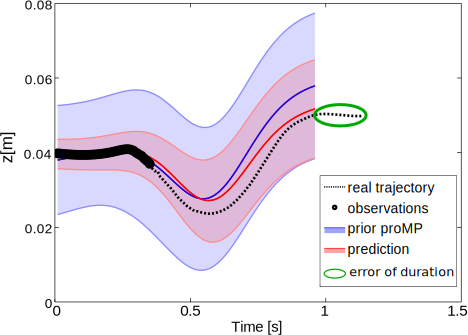
\includegraphics[width=13cm]{img/mean_alpha_errV2.pdf}
\caption{Trajectoire prédite à partir de l'observation d'une trajectoire initiée (points noirs); réalité terrain (\textit{e.g.}, la trajectoire que l'utilisateur voudrait que le robot execute) ; distribution à priori (en bleu clair) ; et distribution postérieur (en rouge), calculée en \toimprove{conditionnant} la distribution afin qu'elle corresponde aux observations. Ici, le calcul de la distribution postérieur est uniquement calculée à partir de la moyenne $\alpha$, de l'ensemble $\alpha_1, \ldots, \alpha_K$ correspondant aux $K$ trajectoires de démonstrations. Sans prédiction du paramètre de modulation du temps de la trajectoire observée et donc en utilisant la moyenne $\alpha$, la trajectoire prédite a une durée visiblement différente de la réalité terrain.}

\label{fig:meanAlpha}
\end{figure}

Durant l'inférence, le paramètre de modulation du temps $\alpha$ de la trajectoire observée partiellement n'est pas connu. À moins que ce paramètre soit fixé à priori, le robot doit alors l'estimer. Cette estimation est essentiel pour assurer une bonne reconnaissance, comme cela est montré dans la Figure~\ref{fig:meanAlpha} : la trajectoire inférée (représentée par la moyenne de la distribution postérieure en rouge) 
%\todo{why "has not the same" is not correct?} 
%For Oriane: check https://english.stackexchange.com/questions/13672/have-not-versus-do-not-have
n'a pas la même durée que la trajectoire attendue ``réelle'' (qui correspond à la réalité terrain). Cette différence est du à l'erreur d'estimation du paramètre de modulation du temps. Cette estimation $\hat{\alpha}$  est calculée par défaut en tant que moyenne de l'ensemble des paramètres $\alpha_k$ calculés lors de la phase d'apprentissage :
\begin{equation}
\label{eq:avg}
%\hat{\alpha} = {1 \over |S_{\alpha k}|} \sum_{\alpha \in S_{\alpha k}} \alpha
\hat{\alpha} = {{\sum \alpha_k} \over n_k} .
\end{equation}

Cependant, l'utilisation de la valeur moyenne du temps de modulation est appropriée uniquement lorsque la primitive représente des mouvements dirigés vers un but très régulier, ou plus généralement lorsqu'il est raisonnable de supposer que les différences de vitesse entre les trajectoires peuvent être négligé (ce qui n'est pas le cas en général). Ainsi, pour beaucoup d'applications, cette estimation est trop imprécise.

C'est pourquoi nous avons trouvé un moyen d'estimer la durée des trajectoires observées, ce qui correspond à estimer de manière précise le paramètre de modulation du temps $\hat{\alpha}$.
Afin d'estimer $\hat{\alpha}$, on a implémenté différentes méthodes.
%Instead, we implemented simpler methods that select the most likely $\hat{\alpha}$ temporal modulation parameter according to different methods.
%\begin{itemize}
%\label{itemize:methodAlphaEstimation}
La première méthode consiste au calcul de la \textbf{moyenne des $\alpha_k$}, comme montré dans l'Équation \ref{eq:avg}. La seconde méthode consiste au calcul du \textbf{maximum de ressemblance }
%As first method, we can simply use the \textbf{mean of the $\alpha$}:
%\begin{equation}
%\label{eq:avg}
%%\hat{\alpha} = {1 \over |S_{\alpha k}|} \sum_{\alpha \in S_{\alpha k}} \alpha
%\hat{\alpha} = {{\sum \alpha_k} \over K} .
%\end{equation}
avec :
\begin{equation}
\label{eq:ml}
\hat{\alpha} = \mathrm{argmax}_{\alpha \in S_{\alpha k}}\{\mathrm{loglikelihood}(\Xi^o,\mu_{\boldsymbol{\omega}_k}, \sigma_{\boldsymbol{\omega}_k}, \alpha_k)\} .
\end{equation} 
La troisième méthode consiste au critère de \textbf{distance minimum}, qui consiste à rechercher le meilleur $\hat{\alpha}$ qui minimise les différences entre la trajectoire observée  $\Xi^o_t$ et celle prédite pour les $n_o$ premières itérations :
\begin{equation}
\label{eq:minDist}
\hat{\alpha} =\mathrm{argmin}_{\alpha \in S_{\alpha k}} \{\sum_{t=1}^{{n_o}} |\Xi^o_t - \Phi_{\alpha t} \mu_{\boldsymbol{\omega}_k}|\} .
\end{equation} 
La quatrième méthode consiste en la création d'un \textbf{modèle}, 
% \todo{find another name}: -> why changing it? the reviewers didnt mind that
basé sur la supposition qu'il y ait une corrélation entre $\alpha$ et la ``variation'' de la trajectoire $\delta_{n_o}$  entre le début et le temps $n_o$. Cette ``variation'' $\delta_{n_o}$ peut correspondre au calcul de la variation positionnelle, \textit{e.g.}, $\delta_{n_o} = X(n_o) - X(1)$,  ou au calcul de la variation de l'ensemble des données représentant la trajectoire, $ \delta_{n_o} =\Xi(n_o) - \Xi(1)$, \toimprove{ou encore n'importe laquelle de ces mesures, tant que l'hypothèse est approprié au type de trajectoire.}\footnote{\toimprove{Dans notre cas, cette hypothèse est appropriée puisque les trajectoires dirigées vers un but de notre application croient généralement de manière monotomne.} }
En effet, le paramètre $\alpha$ peut être lié à la vitesse de mouvement, qui peut être approximée de manière \toimprove{brut} par $\dot{X} ={ \delta X  \over t_f}$ ($\dot{\Xi} ={ \delta \Xi  \over t_f}$). Nous modelisons le réechantillonage entre $\delta_{n_o}$ et $\alpha$ avec : 
\begin{equation}
\label{eq:model}
\alpha = \Psi(\delta_{n_o})^\top \boldsymbol{\omega}_\alpha + \epsilon_\alpha,
\end{equation} 
où $\Psi$ correspond à la matrice de \textit{RBFs}, et $\epsilon_\alpha$ au bruit suivant une loi normale centrée \todo{et réduite ?} .
Lors de la phase d'apprentissage, le paramètre $\boldsymbol{\omega}_\alpha$ est calculé en utilisant l’Équation~\ref{eq:w}. 
Lors de la phase de prédiction, le paramètre $\hat{\alpha} = \Psi(\delta_{n_o})^\top \boldsymbol{\omega}_\alpha$ est calculé.
%\end{itemize}

Une étude test, présentée dans la Section~\ref{sec:simulatedTimeModulationModels}, met en jeu le iCub simulé et permet de comparer ces quatre méthodes d'estimation du paramètre  $\alpha$.

\todo{verif déja inclu dans SOA}
Dans la littérature, il existe d'autres méthodes permettant de calculer ce paramètre $\alpha$. Par exemple~ \cite{ewerton2015learning} propose une méthode qui modélise localement la variabilité de la vitesse d'execution des trajectoires. Dans~\cite{maeda2016probabilistic} ils utilisent une méthode qui permet d'améliorer la méthode \textit{Dynamic Time Warping} en imposant une fonction régulière sur l’alignement temporaire, à l'aide d'optimisation locale. Ces méthodes seront implémentées dans les futures études.
%In this software, we did not implement such methods yet, since the four proposed criteria are simpler.


\subsection{\toimprove{Reconnaître une primitive de mouvement parmi plusieurs}}
\label{sec:ManyProMP}
%
%we learn many movement primitives which correspond to different tasks.\\
%Let  $S_k = \{\Xi_1,\ldots, \Xi_n\}_k$, the set of trajectories that correspond to the $k$-th movement primitive.
%Let recall that $\Xi_i = [\xi_{1} \ldots \xi_{t_{fi}}]^\top$ is the $i$-th trajectory of this data set, where $t_{fi}$ is the final time of the movement. 
%
Pour rendre les robots performant, ceux-ci doivent être capable de proposer différents comportements afin d'effectuer différentes tâches.  Dans notre logiciel, chaque \textit{ProMP} représente une tâche distincte.
Ainsi, il est important que le robot soit capable d'apprendre différentes \textit{ProMPs}, disons $K$, puis d'être capable de reconnaître laquelle de ces trajectoire est initiée par l'utilisateur du robot.
%We are also interested in learning many ProMPs, say $K$ ProMPs.

Durant la phase d'apprentissage d'une Primitive de Mouvement $k \in [1:K]$,  le robot observe différentes trajectoires $S_k = \{\Xi_1,\ldots,\Xi_n\}$. Pour chaque \textit{ProMP}, il apprend alors une distribution à partir de l'ensemble des vecteurs paramètres  $p(\boldsymbol{\omega}) \sim \mathcal{N}(\mu_{\boldsymbol{\omega}_k}, \Sigma_{\boldsymbol{\omega}_k})$, à l'aide de l'Équation~\ref{eq:w}. De plus, le robot enregistre les différentes durées des trajectoires observées : $ S_{\alpha k} = \{\alpha_{1k},\ldots,\alpha_{nk}\}$.

Après avoir apris ces $K$ \textit{ProMPs}, le robot peut utiliser les informations apprises afin d’exécuter une trajectoire et sa tâche correspondante. Pour cela, le robot doit d'abord être capable de reconnaître, à partir des observations partielles de la trajectoire initiée par l'utilisateur, quel est le mouvement et la tâche attendue, puis comment la continuer.
%\todo{why not: has to?} must finish a human-initiated movement on its own. 

Soit $\Xi^{o} = [\Xi_1 \ldots \Xi_{n_o}]^\top$ les observations partielles de la trajectoire initiée.
À partir de ces observations partielles, le robot peut reconnaître la \textit{ProMP} ``correcte'' (\textit{e.g.}, la plus probable) $\hat{k} \in [1:K]$ en suivant plusieurs étapes.
% by:
%\begin{itemize}
Tout d'abord, pour chaque \textit{ProMP} $k \in [1:K]$, le robot commence par calculer le paramètre de modulation de temps $\hat{\alpha}_k$ le plus probable (\textit{c.f.} Section~\ref{sec:predictDuration}), afin d'obtenir un ensemble contenant les \textit{ProMPs} couplées avec leur durée la plus probable : $S_{[\mu_{\boldsymbol{\omega}_k}, \hat{\alpha}_k]} = \{(\mu_{\boldsymbol{\omega}_1},\hat{\alpha}_1),\ldots,(\mu_{\boldsymbol{\omega}_K},\hat{\alpha}_K)\}$

Puis, le robot calcul la \textit{ProMP} $\hat{k}$ la plus probable depuis l'ensemble : $S_{[\mu_{\boldsymbol{\omega}_k}, \hat{\alpha}_k]}$, en utilisant différents critères. \todo{?}
Afin de minimiser la distance entre les observations partielles et la moyenne des premières données de la \textit{ProMP}, le robot peut calculer :
\begin{equation} \label{eq:mostlikelypromp}
\hat{k} = \arg \min_{k \in [1:K]} \,   \left[      {1 \over n_o} \sum_{t=1}^{n_o}| \Xi_{t} - \Phi_{\hat{\alpha}_k t} \, \mu_{\boldsymbol{\omega}_k} | \right]
\end{equation}
Dans l'Équation~\ref{eq:mostlikelypromp}, pour chaque \textit{ProMP}  $k \in [1:K]$, la distance moyenne est calculée entre la trajectoire initiée $\Xi_t$  et la moyenne de la \textit{ProMP} $\Phi_{\hat{\alpha}_k t} \mu_{\omega_k}$, avec $t = [1:n_o]$.
La \textit{ProMP} $\hat{k}$ la plus vraissemblable est alors selectionnée en calculant la distance minimum (arg min). D'autres méthodes sont possibles pour calculer la \textit{ProMP} la plus probable, méthodes inspirées par celles présentées pour l'estimation du paramètre de modulation du temps ( \textit{c.f.} Section précédente). C'est à dire, l'estimation à l'aide du maximum de vraisemblance ou en apprenant une modélisation du paramètre, \toimprove{modèle basée sur des données de la trajectoire}.

%\end{itemize}
%\todo{EXPLAIN THIS EQUATION}

%Now the ProMP the most similar to the early-trajectory is identified, we can update the $\hat{k}$-th ProMP to adapt it to the observed early-trajectory.

Lorsque la $\hat{k^e}$ \textit{ProMP} la plus probable a été identifiée, la distribution postérieure de cette \textit{ProMP} est caclulée afin de prendre en compte la portion initiale de la trajectoire observée, en utilisant l'Équation~\ref{eq:inf}:

%The first step is then to compute $\hat{t_f}$ \rev{(the expected duration of the trajectory)} by: 
%\begin{equation}
%\hat{t_f} = \hat{\alpha_{\hat{k}}} \times \bar{s}
%\end{equation}
%The second step consists of updating the ProMP to match the early observations, using Equation~\ref{eq:inf}:

%\hat{\alpha}_{\hat{k}}
%\omega}_{\hat{k}}
\begin{equation} \label{eq:udateWithAlpha}
\left\{
\begin{array}{rl}
\hat{\mu}_{\boldsymbol{\omega}_{\hat{k}}} &= \mu_{\boldsymbol{\omega}_{\hat{k}}}  + K(\Xi^o - \Phi_{\hat{\alpha}_{\hat{k}}[1:{n_o}]}\mu_{\boldsymbol{\omega}_{\hat{k}}} ) \\ 
\hat{\Sigma}_{\boldsymbol{\omega}_{\hat{k}}}  &= \Sigma_{\boldsymbol{\omega}_{\hat{k}}}  - K(\Phi_{\hat{\alpha}_{\hat{k}}[1:{n_o}]} \Sigma_{\boldsymbol{\omega}_{\hat{k}}} ) \\
K&= \Sigma_{\boldsymbol{\omega}_{\hat{k}}} \, \Phi_{\hat{\alpha}_{\hat{k}}[1:{n_o}]}^\top \, (\Sigma_{\xi^o} + \Phi_{\hat{\alpha}_{\hat{k}}[1:n_o]}\Sigma_{\boldsymbol{\omega}_{\hat{k}}}  \Phi_{\hat{\alpha}_{\hat{k}}[1:n_o]}^\top)^{-1}
\end{array}
\right.
\end{equation}
avec $\hat{\alpha}_{\hat{k}}[1:n_o] = \hat{\alpha}_{\hat{k}} \, t$ (forme matricielle), avec $t \in [1:n_o]$.

Finalement, la trajectoire inférée est calculée avec : 
$$\forall t \in [1:\hat{t}_f], \hat{\xi}(t) = \Phi_t \, \hat{\mu}_{\boldsymbol{\omega}_{\hat{k}}}$$
avec une estimation de la durée de la trajectoire correspondant à : $\hat{t}_f = \hat{\alpha}_k\bar{s}$.
Le robot est alors capable de finir le mouvement en executant la trajectoire ``future'' la plus probable : $\hat{\Xi} =[\hat{\xi}_{n_o+1} \ldots \hat{\xi}_{\hat{t_{f}}}]^\top$.


%\newpage
%%%%%%%%%%%%%%%%%%%%%%%%%%%%%%%%%%%%%%%%%%%%%%%%%%%%%%%%%%%%%%%%%%%%%%%%%%%%%%%%
\section{Présentation du logiciel}\label{sec:softwareOverview}

Dans cette Section, le logiciel libre d'accès est présentée. Ce logiciel est composé de deux modules, représentés dans la Figure \ref{fig:orgaSoftware}.

\label{sec:software}
\begin{figure}[h]
\center
\includegraphics[width=\hsize]{img/liaisonAllProgramV3.pdf}
\caption{Architecture du logiciel avec représentation des échanges de donées.\\ Le contrôle du robot est soit guidé par son utilisateur (manuellement ou à l'aide d'un dispositif haptique) représenté en bleu, ou à l'aide d'un module Matlab, présenté en violet. \toimprove{Le module  C++ permet de faire passer l'information de contrôle à la commande robotique, comme présenté en noir}. De plus, ce module transmet l'information qui provient du \textit{iCub}.}
\label{fig:orgaSoftware}
\end{figure}

Durant la phase d'apprentissage, où le robot apprend les différentes \textit{ProMPs} et leur tâche correspondante, le robot est contrôlé par un utilisateur. Celui-ci peut guider le robot manuellement, lorsqu'il s'agit du \textit{iCub} réel, ou à l'aide d'un dispositif haptique lorsqu'il s'agit de la simulation du robot.

Un module Matlab permet de rejouer les \textit{ProMPs}, ou de finir un mouvement qui a été initié par son utilisateur. Ce module permet au robot d'apprendre des \textit{ProMPs} à partir des trajectoires effectuées; de rejouer ces \textit{ProMPs}; de reconnaître la \textit{ProMP} qui correspond le plus à une trajectoire en cours; et de prédire le ``futur'' de cette trajectoire, jusqu'à atteindre le but.
%\todo{and to make sure that the user's forces exerted on the robot are not stronger than the ones learnt.}

Un module C++ transmet au robot l'information de contrôle qui provient soit de l'utilisateur, soit du module Matlab. Le robot est alors capable de finaliser le mouvement inité par son utilisateur (directement ou à l'aide d'un dispositif haptique) de manière autonome, comme présenté dans la Figure~\ref{fig:conceptProMP}. %\todo{This program communication also allows to correct the robot behaviour if the users forces are stronger than the expected ones.} \\
Le module C++ est présenté dans la Section~\ref{subec:Setup}, puis une explication théorique des algorithmes utilisés dans le module Matlab  est donnée dans la Section~\ref{sec:theory}. Un guide permettant d'utiliser ce module Matlab est d'abord présenté dans  la Section~\ref{sec:example1DOF} dans le cas d'un exemple jouet, puis dans la Section~\ref{sec:3ProMPsAppli} dans le cas de notre application, où le robot simulé apprend différentes données sur les mouvements (\textit{e.g.}, il s'agit de \textit{ProMPs} à plus haute dimension). Finalement, les résultats de l'application effectué sur le réel robot \textit{iCub} sont présentés dans la Section~\ref{sec:appliRealIcub}.

Notre logiciel est disponible avec une licence GPL, et est accessible publiquement à l'adresse : 

\url{https://github.com/inria-larsen/icubLearningTrajectories}.

Ce répertoire propose à la fois un tutoriel, un fichier d'explication (README) et des vidéos de présentation.
Le fichier d'explication décrit comment lancer des démonstrations basiques. Les vidéos présentent ces démonstrations, afin d'éclaircir le fonctionnement de cette application. Les sections prochaines détaillerons tout d'abord comment fonctionne le ``programme de démonstration'' disponible, permettant l'apprentissage d'une primitive à une dimension; suivi par la présentation d'une application spécifique au \textit{iCub} (d'abord en simulation puis sur le robot réel).
%\todo{check that, it is not in the readme??}


%%%%%%%%%%%%%%%%%%%%%%%%%%%%%%%%%%%%%%%%%%%%%%%%%%%%%%%%%%%%%%%%%%%%%%%%%%%%%%%%
\section{Software example: learning a 1-DOF primitive}
\label{sec:example1DOF}
\rev{In this section, we present the use of the software to learn ProMPs in a simple case of 1-DOF primitive. This example only uses the \textit{MatlabProgram} folder, composed of:}
\begin{itemize}
\item A sub-folder called ``Data'', where \rev{there are trajectory sets used to learn movement primitives. These trajectories are stored in text files with the following information}:
%that
%\sout{there are some samples of trajectories in text files. These text files} }can be organize in various ways:
\begin{itemize}
\item [-] \textbf{input parameters}: \# input$_1$ \# input$_2$ [...]
\item [-] \textbf{input parameters with time-step}: \# timeStep \# input$_1$ \# input$_2$ [...]
\item [-] \textbf{\textit{recordTrajectories.cpp} program recording}: See Section~\ref{sec:dataAquisition} for more information.
\end{itemize}
\item A sub-folder called ``used\_functions''. It contains all the functions used to retrieve trajectories, compute ProMPs, infer trajectories, and plot results. Normally, \rev{using this toolbox does not require understanding these functions. }
%\sout{the use of this toolbox doesn't require to understand these functions}}. 
The first lines of these functions give an explanation of \rev{their} functioning and precise what are the input(s) and output(s) parameters.
\item Matlab scripts called ``demo\_*.m". They are simple examples of how to use this toolbox.
\end{itemize}

<<<<<<< HEAD
The script \mcode{demo\_plot1DOF.m}, can be used to compute a ProMP and to continue an initiated movement. The ProMP is computed from a dataset stored in a ".mat" file, called \textit{traj1\_1DOF.mat}. In this script, variables are first defined to make the script specific to the current dataset:
\begin{tabular}{|c|l|}
  \hline
  \textbf{Variable assignation} & \textbf{Commentary}\\
  \hline
  DataPath\= 'Data\/traj1\_1DOF.mat'; & Can be either ".mat" or ".txt". In the current demo,  you can also write\\
  & DataPath $=$ 'Data/traj1' if you want to use the text files of this dataset.\\
     \hline
  typeRecover= '.mat' & Or .txt, it depends on your choice of data file.\\
    \hline
  inputName = {'z[m]'}; & Label of your input(s). Here $z$ represents the $z$-axis Cartesian coordinate.\\
    \hline
  s\_ref=100; & Number of samples used as reference to rescale all the trajectories.\\
  & to the same duration.\\
    \hline
  nbInput = 1; & Dimension of the generic vector containing the state of the trajectory.\\
    \hline
  M = 5;  & Number of radial basis functions per input.\\
    \hline
  expNoise = 0.00001;  & Expected trajectory noise.\\
    \hline
  percentData = 20;  & Percent of observed data during the inference.\\
  \hline
  \end{tabular}

The variables include:
\begin{itemize}
\item \mcode{DataPath} is the path to the recorded data. If the data are stored in text files, this variable contains the folder name where text files are stored. These text files are called ``record$X$.txt", with $X \in [0:n-1]$ if there are $n$ trajectories. One folder is used to learn one ProMP. If the data are already loaded from a ``.mat" file, write the whole path with the extension. The data in ``.mat" matches with the output of the Matlab function \mcode{loadTrajectory}. %, presented in Figure~\ref{fig:yobject}.
\item \mcode{nbInput}= $D$ is the dimension of the input vector $\xi_t$. 
%This variable can be divided in two to precise in \mcode{nbInput(1)} what are the first $\xi_t$  dimensions used to recognize both the correct movement primitive and the time modulation of the initiated trajectory. In that case, \mcode{nbInput(2)}$= D - $\mcode{nbInput(1)}, contains the other dimensions, only used to compute the posterior distribution.
\item \mcode{expNoise} $= \Sigma^o_\xi$ is the expected noise of the initiated trajectory. The smaller this variable is, the stronger the modification of the ProMP distribution will be, given new observations.
\end{itemize}

%\rev{After this variable declaration, the user can just launch the script. To give a deeper understanding of this script, we now detail which and how functions are called in it.} 
We will now explain more in detail the script. 
To recover data recorded in a ``.txt'' file, we call the function:

\mcode{t\{1\} = loadTrajectory(PATH, nameT, varargin)} 

Its input parameters specify the path of the recorded data, the label of the trajectory. Other information can be added by using the \mcode{varargin} variable (for more detail, check the header of the function with the help comments). 
%For more detail about these parameters, read the beginning of this function. 
The output is an object that contains all the information about the demonstrated trajectories. \rev{It is composed of \mcode{nbTraj}, the number of trajectory; \mcode{realTime}, the simulation time; \mcode{y} (and \mcode{yMat}), the vector (and matrix) trajectory set , etc.}. 
%\rev{\sout{Note that to simplify the Matlab's notation, we denote the $\Xi$ trajectory by \mcode{y} (or \mcode{yMat} in all the toolbox functions}}. 
\rev{Thus, \mcode{t\{1\}.y\{i\} } contains the $i$-th trajectory}.

%\begin{figure}[h]
%\centering
%\includegraphics[height=4cm]{img/yobject.pdf}
%\caption{Object that contains information about 51 observed trajectories of a 1DOF movement primitive.}
%\label{fig:yobject}
%\end{figure}

The Matlab function \mcode{drawRecoverData(t\{1\}, inputName,'namFig', nFig, varargin)} plots in a Matlab figure (numbered \mcode{nFig}) the dataset of loaded trajectories. %By lack of place, we don't represent here these trajectories.
\rev{An example is shown in Figure~\ref{fig:1DOFtrajectoriesProMP}, on the left. Incidentally, the different duration of the trajectories is visible: on average, it is $1.17 \pm 0.42$ seconds.}

% a plot such as Figure~\ref{fig:1DOFtrajectories}. In this Figure, the average duration of these trajectories is $1.17 \pm 0.42$ seconds.

%\begin{figure}[h]
%\centering
%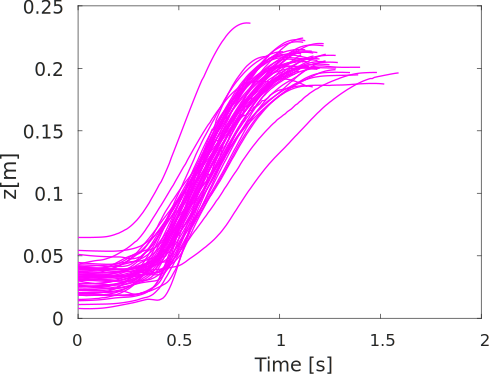
\includegraphics[height=8cm]{img/1DOFtrajectoriesV2.pdf}
%\caption{The trajectories of the test dataset for 1DOF primitive.}
%\label{fig:1DOFtrajectories}
%\end{figure}

To split the \rev{entire dataset of demonstrated} trajectories \mcode{t\{1\}} 
into a training dataset (used for learning the ProMPs) and a test dataset (used for the inference), call the function

\mcode{[train, test] =  partitionTrajectory(t\{1\}, partitionType, percentData, s_ref)}
\rev{where if \mcode{partitionType}$=1$, only one trajectory is in the test set and the others are placed in the training set, and if \mcode{partitionType}$ >1$ it corresponds to the percentage of trajectories that will be included in the training set.} 
%\rev{\sout{
%where \mcode{percentTrain} is the percentage of trajectories that \rev{will be included \sout{goes}} in the training \rev{\sout{data}}set. If \mcode{percentTrain=1}, only one trajectory is randomly selected to be in the inference dataset.}}

\rev{The ProMP can be computed from the training set by using the function}:

\mcode{promp = computeDistribution(train, M, s_ref,c,h)}

The output variable \mcode{promp} is an object that contains all the ProMP information. 
The first three input parameters have been presented before: \rev{\mcode{train} is the training set, \mcode{M} is the number of \textit{RBFs}, \mcode{s_ref} is the number of samples used to rescale all the trajectories.}
The last two input parameters \mcode{c} and \mcode{h} shape the \textit{RBFs} of the ProMP model: \mcode{c} $\in \mathbb{R}^M$ is the center of the Gaussians and \mcode{h} $\in \mathbb{R}$ their variance. 

%In Matlab, the equivalent code is:
%\begin{lstlisting}
%for i = 1:3
%	if i >= 5 && a ~= b       % literate programming replacement
%		disp('cool');           % comment 
%	MATLAB CODE
%end
%\end{lstlisting}
%\todo{I don't get here what you want I write: to c/p the program will be to long. DO you want I do a pseudo-code?}
To visualize this ProMP, as shown in Figure~\ref{fig:1DOFtrajectoriesProMP}, call the function:
\mcode{drawDistribution(promp, inputName,s_ref)}



\begin{figure}[h]
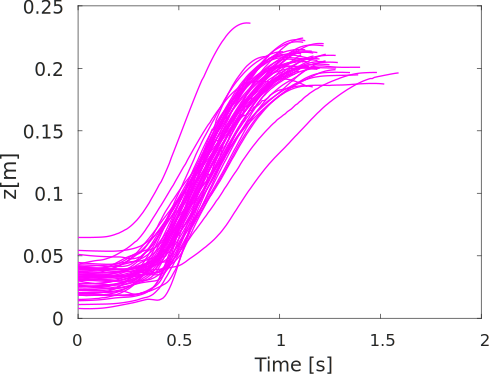
\includegraphics[width=\hsize /2]{img/1DOFtrajectoriesV2.pdf} 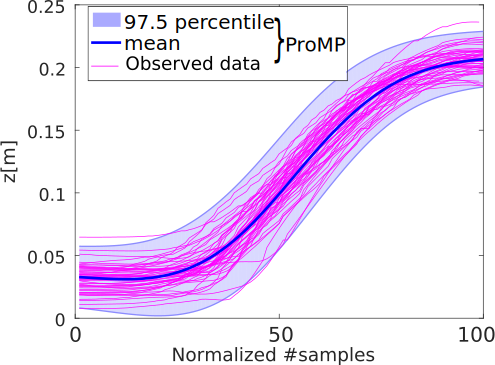
\includegraphics[width=\hsize /2]{img/1DOFtrajectoriesProMPV2.pdf}
%\caption{The trajectories of the test dataset for 1DOF primitive.}
\caption{The observed trajectories are represented in magenta. The corresponding ProMP is represented in blue. The following parameters are used: $\bar{s}=100$ for the reference number of samples, $M=5$ for the number of \textit{RBFs} spread over time, and  $h=0.04$ (=$ 1 \over M^2$) the variance of the \textit{RBFs}.}
\label{fig:1DOFtrajectoriesProMP}
\end{figure}

%In this figure, the distribution is represented according to a reference number of samples $\bar{s} = 100$, and the observed trajectory are resaled according to this number of samples, to facilitate the understanding.

For debugging purposes and to understand how to tune the ProMPs' parameters, it is interesting to plot the overlay of the basis functions in time. Choosing an appropriate number of basis functions is important, as too few may be insufficient to approximate the trajectories under consideration, and too many could result in over-fitting problems.
To plot the basis functions, simply call: 

\mcode{drawBasisFunction(promp.PHI,M)}

where \mcode{promp.PHI} is a set of \textit{RBFs} evaluated in the normalized time range $t \in [1:\bar{s}]$.
%, each of which being evaluated at a different time $t \in [1:\bar{s}]$. \todo{is it better?}%during the interval: $\Phi_{[1:\bar{s}]}$ \todo{reformulate this}. 

Figure \ref{fig:1DOFtrajectoriesProMPbasis} shows at the top the basis functions before normalization, and at the bottom the ProMP modeled from these basis functions. From left to right, we change the number of basis functions. When there are not enough basis functions (left), the model is not able to correctly represent the shape of the trajectories. In the middle, the trajectories are well represented by the five basis functions. With more basis functions (right), the variance of the distribution decreases because the model is more accurate. 
\rev{However, arbitrarily increasing the number of basis functions is not a good idea, as it may not improve the accuracy of the model and worse it may cause overfitting. }
%\rev{With too many basis function, there is no real improvement of the accuracy and it may be overfitting}.
%As a balance, the computation time increases.

\begin{figure}[h]
\centering
{
\includegraphics[width=\hsize]{img/1DOFtrajectoriesProMPbasisV4.pdf}
}
\caption{The ProMP computed for the test dataset (Figure \ref{fig:1DOFtrajectoriesProMP}) using different numbers of basis functions: from left to right: $M=\{2,5,50\}$ basis functions before normalization, with a variance $h={1 \over M^2}$. }
\label{fig:1DOFtrajectoriesProMPbasis}
\end{figure}

Once the ProMP is learned, the robot can reproduce the movement primitive using the mean of the distribution.
Moreover, it can now recognize a movement that has been initiated in this distribution, and predict how to finish it. To do so, given the early $n_{o}$ observations of a movement, the robot updates the prior distribution to match the early observed data points: through conditioning, it finds the posterior distribution, that can be used by the robot to execute the movement on its own.

The first step in predicting the evolution of the trajectory is to infer the duration of this trajectory, which is encoded by the time modulation parameter $\hat{\alpha}$. The computation of this inference, which was detailed in Section~\ref{sec:predictDuration}, can be done by using the function:

\mcode{[expAlpha,type,x]=inferenceAlpha(promp,test\{1\},M,s_ref,c,h,test\{1\}.nbData, expNoise, typeReco)}

where \mcode{typeReco} is the type of criteria used to find the expected time modulation ('MO', 'DI' or 'ML' for model, distance or maximum likelihood methods); \mcode{expAlpha} $=\hat{\alpha}$ is the expected time modulation; \mcode{type} is the index of the ProMP from which \mcode{expAlpha} has been computed, which we note in this paper as $k$ .
%\mcode{x} is used for debugging purpose.
%\marco{Finally \mcode{x = test\{1\} + offset} is the trajectory transposed by an offset, to be centred on the mean of the recognized ProMP at time $t=1$ (only used for debugging purposes).[Obs.: I didn’t understand
%584 this.] }
%\rev{it is hard to explain in the paper, but from the early-trajectory, to recognize which ProMPs correspond the best to the initiated trajectory, I need to translate the early-trajectory to compute how likely the "shape" of the early-trajectory correspond to the ProMP}
To predict the evolution of the trajectory, we use Equation~\ref{eq:inf} from Section \ref{sec:predict}. In Matlab, this is done by the function:
\mcode{infTraj = inference(promp, test\{1\}, M, s_ref, c, h, test\{1\}.nbData, expNoise, expAlpha)}\\
where \mcode{test\{1\}.nbData} has been computed during the \mcode{partitionTrajectory} step. This variable is the number of observations $n_o$, representing the percentage of observed data (\mcode{percentData}) of the test trajectory (\textit{i.e.}, to be inferred) that the robot observes. \mcode{infTraj}$= \hat{\Xi}$ is the inferred trajectory.
Finally, to draw the inferred trajectory, we can call the function  \mcode{drawInference(promp,inputName,infTraj, test{1},s_ref)}.

It can be interesting to plot the quality of the predicted trajectories as a function of the number of observations, as done in Figure \ref{fig:1DOFtrajectoriesPredictions}.

\begin{figure}[h]
\centering
{
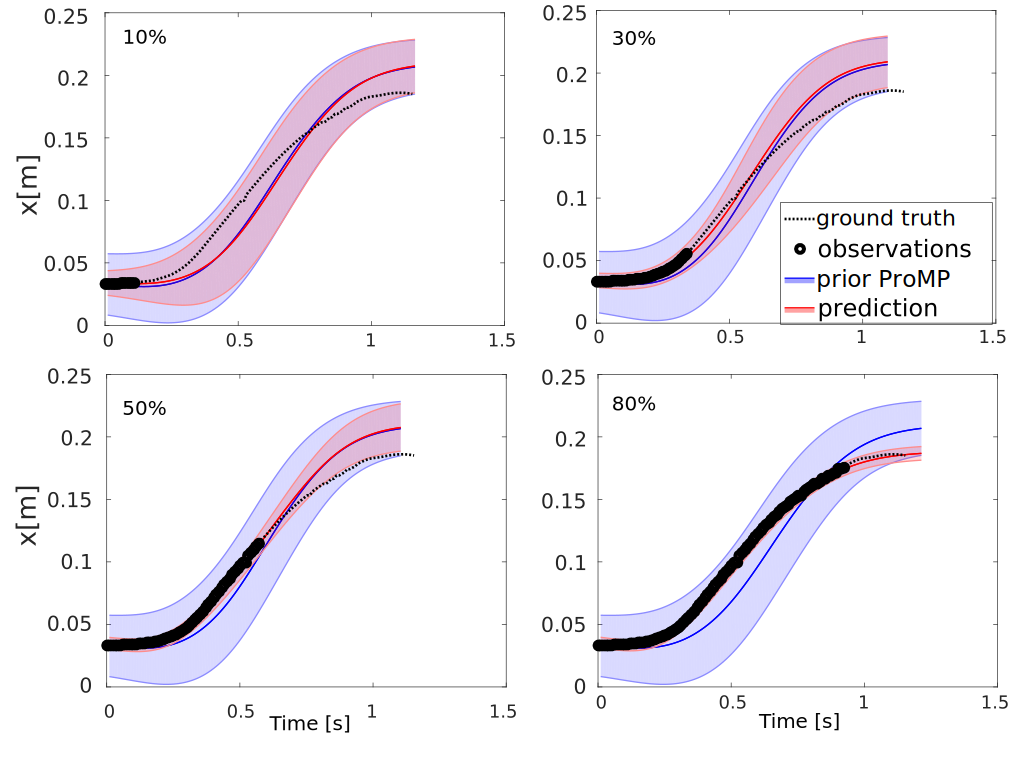
\includegraphics[width=15cm]{img/1DOFtrajectoriesPredictionsV2.pdf}
}
\caption{The prediction of the future trajectory given early observations, exploiting the information of the learned ProMP (Figure \ref{fig:1DOFtrajectoriesProMP}). The plots show the predicted trajectories after 10\%, 30\%, 50\% and 80\% of observed data points.}
% \marco{[This paper explained how to compute the posterior over $\omega$, but not how to
%compute the prior nor the posterior over trajectories. However this must be computed somewhere
%to generate figures such as this one.]} \rev{I don't understand, in eq~\ref{eq:w} we explain how the prior is computed}}
\label{fig:1DOFtrajectoriesPredictions}
\end{figure}

Note that when we have \rev{observed a larger portion of the trajectory, the prediction of the remaining portion is more accurate}.

Now we want to measure the quality of the prediction. Let $\Xi^* = [\xi^o(1),\ldots, \xi^o({n_o}), \xi^*(n_o+1),\ldots, \xi^*(t^*_f)]$ be the real trajectory expected by the user. 
To measure the quality of the prediction, we can use:
\begin{itemize}
\item The likelihood of having the $\Xi^*$ trajectory given the updated distribution $\hat{p(\boldsymbol{\omega})}$.
\item The distance between the $\Xi^*$ trajectory and the  $\hat{\Xi}$ inferred trajectory.
\end{itemize}

However, according to the type of recognition \mcode{typeReco} used to estimate the time modulation parameter $\alpha$ from the early observations, a visible mismatch between the predicted trajectory and the real one can be visible even when a lot of observations are used. This is due to the error of the expectation of this time modulation parameter. In Section \ref{sec:predictDuration}, we present the different methods used to predict the trajectory duration. These methods select the most likely $\hat{\alpha}$ according to different criteria: distance; maximum likelihood; model of the $\alpha$ variable\footnote{In this model, we assume that we can find the time modulation parameter according to the global variation of the position during the $n_o$ first observed data.}; and average of the observed $\alpha$ during learning.
%
%\todo{Je ne pense pas mettre l'exemple ci dessous que tu souhaitais parce que le code est assez long. \\
%In Matlab, this further prediction can be done by:}
%
%\begin{lstlisting}
%for i = 1:3
%	if i >= 5 && a ~= b       % literate programming replacement
%		disp('cool');           % comment 
%	MATLAB CODE
%end
%\end{lstlisting}

Figure \ref{fig:1DOFtrajectoriesPredictionsDuration} shows the different trajectories predicted after $n_{o}=40\%$ of the length of the desired trajectory is observed, according to the method used to estimate the time modulation parameter. 

On this simple test, where the variation time is little as shown in Table \ref{tab:alphaProMP}, the best result is accomplished by the average of time modulation parameter of the trajectories used during the learning step. In more complicated cases, when the time modulation varies, the other methods will be preferable as seen in Section~\ref{sec:ManyProMP}.
\begin{table}
\center
\begin{tabular}{|p{2.5cm}|p{2.5cm}|p{4.5cm}|p{2.5cm}|}
  \hline
    & Traj. Samples & $\alpha = {\bar{s} \over \mathrm{Iterations}}, \bar{s}=100$ & Duration [s] \\
     \hline
     Min & 83 & 1.2048 & 0.83 \\
     \hline
     Max & 115 & 0.8696 & 1.15\\
     \hline
     Mean & 100& 1& 0.99 \\
     \hline
     Std deviation & 9 & 11.1111 & 0.09 \\
     \hline
\end{tabular}
\caption{information about trajectories' duration}
\label{tab:alphaProMP}
\end{table} 

\begin{figure}[h]
\centering
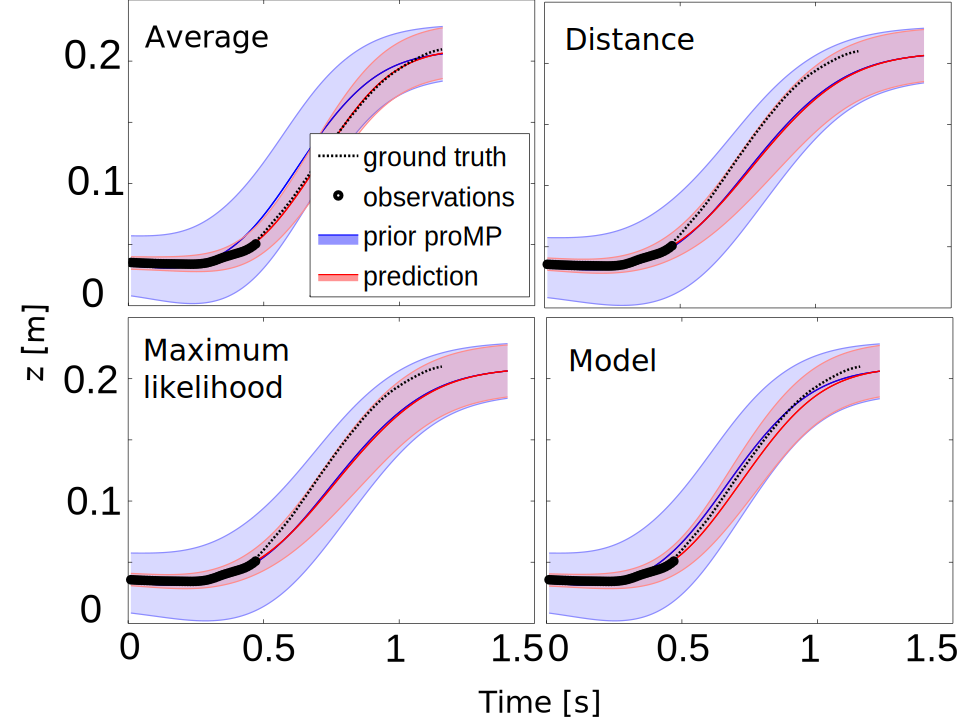
\includegraphics[width=15cm]{img/1DOFtrajectoriesPredictionsDurationV2.pdf}
\caption{The prediction of the future trajectory given $n_{o}=40\%$ of early observations from the learned ProMP computed for the test dataset (Figure \ref{fig:1DOFtrajectoriesProMP}). The plots show the predicted trajectory, using different criteria to estimate the best phases of the trajectory: using the average time modulation (Equation~\ref{eq:avg}); using the distance criteria (Equation~\ref{eq:minDist}); using the maximum log-likelihood (Equation~\ref{eq:ml}); or using a model of time modulation according to the time variation (Equation~\ref{eq:model}).}
\label{fig:1DOFtrajectoriesPredictionsDuration}
\end{figure}


%%%%%%%%%%%%%%%%%%%%%%%%%%%%%%%%%%%%%%%%%%%%%%%%%%%%%%%%%%%%%%%%%%%%%%%%%%%%%%%%
\section{Application on the simulated iCub: learning three primitives}
\label{sec:3ProMPsAppli}
\begin{figure}[h]
\centering
{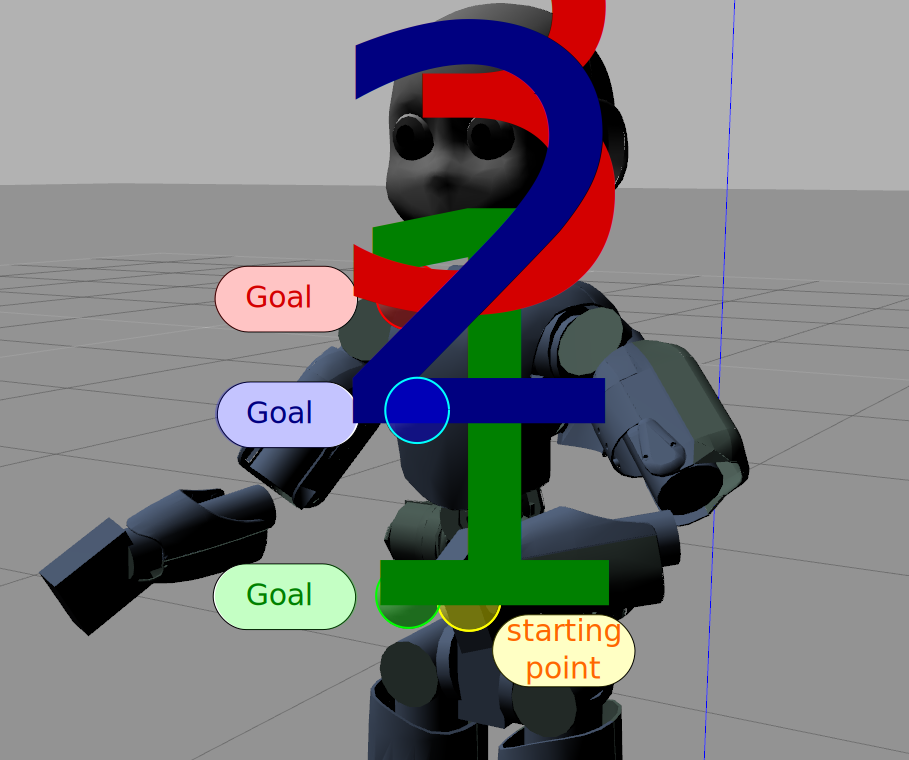
\includegraphics[width=8cm]{img/gazeboGoalsV2.pdf}
\hspace{0.1cm}
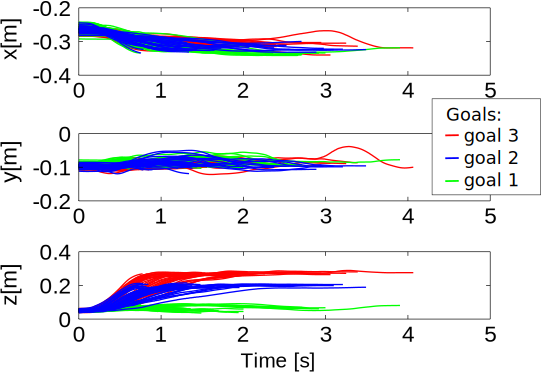
\includegraphics[width=9cm]{img/3DOFtrajectories.pdf}
}
\caption{Left: the three colored targets that the robot must reach from the starting point; the corresponding trajectories are used to learn three primitives representing three skills. 
Right: the Cartesian position information of the demonstrated trajectories for the three reaching tasks.}% trajectories x (top),y(middle) and(bottom) without force information that are also recorded.}
\label{fig:3TargetsTrajectories}
\label{fig:GazeboGoal}
\end{figure}

In this application, the robot learns multiple ProMPs and is able to predict the future trajectory of a movement initiated by the user, assuming the movement belongs to one of the learned primitives. Based on this prediction, it can also complete the movement once it has recognized the appropriate ProMP. 

We simplify the three actions/tasks by reaching three different targets, represented by three colored balls in the reachable workspace of the iCub. The example is performed with the simulated iCub in Gazebo. Figure~\ref{fig:GazeboGoal} shows the three targets, placed at different heights in front of the robot.

In Section~\ref{sec:formulateModelInt} we formulate the intention recognition problem for the iCub: the problem is to learn the ProMP from trajectories consisting of Cartesian positions in 3D\footnote{Note that in that particular example we do not use the orientation because we want the robot's hand to keep the same orientation during the movement. But in principle, it is possible to learn trajectories consisting of the 6D/7D Cartesian position and orientation of the hand, to make the robot change also the orientation of the hand during the task.} and the 6D wrench information measured by the robot during the movement.
In Section \ref{subec:Setup} we describe the simulated setup of iCub in Gazebo, then in Section~\ref{sec:dataAquisition} we explain how trajectories are recorded, including force information, when we use the simulated robot.


\subsection{Predicting intended trajectories by using ProMPs}\label{sec:formulateModelInt}

The model is based on Section~\ref{sec:theory}, but here we want to learn more information during movements. We record this information \rev{in} a multivariate parameter vector:
$$\forall t, \xi_t=\begin{bmatrix} X_t \\ F_t\end{bmatrix} \in \mathbb{R}^{9}$$ 
Were $X_t \in \mathbb{R}^{3}$ is the Cartesian position of the robot's end effector and $F_t \in \mathbb{R}^6$ the external forces and moments. In particular, $F_t$ contains the user's contact forces and moments. Let us call dim($\xi_t$)$ = D$, the dimension of this parameter vector. %Let $\xi_{inf} =[\xi_{o+1} \ldots \xi_{t_{f}}]^\top$ the output vector of the expected end trajectory, where $t_f$ is the expected total time of the movement.

The corresponding ProMP model is:
$$\xi_t = \begin{bmatrix} X_t \\ F_t\end{bmatrix} = \Phi_{\alpha t} \boldsymbol{\omega} + \epsilon_t$$
Where $\boldsymbol{\omega} \in  \mathbb{R}^{D \cdot M}$ is the time independent parameter vector, $\epsilon_t= \begin{bmatrix} \epsilon_{X_t} \\ \epsilon_{F_t}\end{bmatrix} \in \mathbb{R}^D$ is the zero-mean Gaussian i.i.d. observation noise, and $\Phi_{\alpha t} \in \mathbb{R}^{D \times D \cdot M}$ a matrix of Radial Basis Functions (\textit{RBFs}) evaluated at time $\alpha t$.\\
Since we are in the multidimensional case, this $\Phi_{\alpha t}$ block diagonal matrix is defined as:
$$\Phi_{\alpha t}  = BlockdiagonalMatrix(\phi_1,\ldots,\phi_{D}) \in \mathbb{R}^{D \times D \cdot M} $$
%\left[ \begin{array}{cccc}
% & \hfill & \hfill & \hfill\\
%\hfill & \phi_\xi & \hfill & \hfill\\
%\hfill & \hfill & \ldots &\hfill \\
%\hfill & \hfill & \hfill & \phi_{m_z}
%\end{array} \right] $
It is a diagonal matrix of $D$ Radial Basis Functions (\textit{RBFs}), where each \textit{RBF} represents one dimension of the $\xi_t$ vector and it is composed of $M$ Gaussians, spread over  same number of samples $\bar{s}$.


\subsubsection{Learning motion primitives}
\label{learning}
%Assume the robot has to learn $K$ movement primitives.\\

During the learning step of each movement primitive $k \in [1:3]$, the robot observes different trajectories $S_k = \{\Xi_1,\ldots, \Xi_n\}_k$, as presented in Section~\ref{sec:dataAquisition}.\\
For each trajectory $\Xi_{i {[1:t_{fi}]}} = [\xi_{i(1)}, \ldots, \xi_{i(tf_i)}]^\top$, it computes the optimal $\boldsymbol{\omega}_{ki}$ parameter vector that best approximates the trajectory.

We saw in Section~\ref{sec:ManyProMP} how these computations are done. In our software, we use matrix computation instead of $t_{fi}$ iterative ones done for each observation $t$ (as in Equation ~\ref{eq:w}). Thus, we have:
\begin{eqnarray}
\boldsymbol{\omega}_{ki} = (\Phi_{\alpha [1:t_{fi}]}^\top \Phi_{\alpha [1:t_{fi}]})^{-1} \Phi_{\alpha [1:t_{fi}]}^\top * \Xi_{i {[1:t_{fi}]}}
\end{eqnarray}
with $\Phi_{\alpha [1:t_{fi}]} = [\Phi_{\alpha 1}, \Phi_{\alpha 2}\ldots,\Phi_{\alpha t_{fi}}]^\top$.


\subsubsection{Prediction of the trajectory evolution from initial observations}
\label{prediction}

After having learned the three ProMPs, the robot \rev{is able to} finish an initiated movement on its own. In Sections~\ref{sec:predict}, \ref{sec:predictDuration} and \ref{sec:ManyProMP} we explained how \rev{to compute the future intended trajectory given the early observations}. %the end of this movement is computed.

In this example, we add specificities about the parameters to learn.

Let $\Xi^{o} = \begin{bmatrix} X^o \\ F^o \end{bmatrix} = [\Xi_1 \ldots \Xi_{n_o}]^\top$ be the early observations of the trajectory.

First, we only consider the partial observations: $X^{o} = [X_1 \ldots X_{n_o}]^\top$.
Indeed, we assume the recognition of a trajectory is done with Cartesian position information only, because the same movement can be done and recognized with different force profiles than the learned ones.

From this partial observation $X^o$, the robot recognizes the current ProMP $\hat{k} \in [1:3]$, as seen in Section~\ref{sec:ManyProMP}. It also computes an expectation of the time modulation $\hat{t}_f$, as seen in Section \ref{sec:predictDuration}. Using the expected value of the time modulation, it approximates the trajectory speed and its total time duration.
%\marco{is this expectation in sense of expected value?}
%\rev{yes}

Second, we use the total observation $\Xi^o$ to update the ProMP, as seen in Section \ref{sec:predict}. This computation is based on equation~\ref{eq:udateWithAlpha}, but here again, we use matrix computation:
$$\left\{
\begin{array}{rl}
\hat{\mu}_{\boldsymbol{\omega}_k} &= \mu_{\boldsymbol{\omega}_k}  + K(\Xi^o - \Phi_{\alpha[1:n_o]} \mu_{\boldsymbol{\omega}_k} ) \\ 
\hat{\Sigma}_{\boldsymbol{\omega}_k}  &= \Sigma_{\boldsymbol{\omega}_k}  - K(\Phi_{\alpha[1:n_o]}\Sigma_{\boldsymbol{\omega}_k} ) \\
K&= \Sigma_{\boldsymbol{\omega}_k} \Phi_{\alpha[1:n_o]}^\top(\Sigma_{\xi^o} + \Phi_{\alpha[1:n_o]}\Sigma_{\boldsymbol{\omega}_k}  \Phi_{\alpha[1:n_o]}^\top)^{-1}
\end{array}
\right.$$

From this posterior distribution, we retrieve the inferred  $\hat{\Xi} = \{ \hat{\xi}_1,..., \hat{\xi}_{\hat{t}_f}\}$ trajectory, with:
$$ \forall t \in [1:\hat{t}_f],\hat{\xi}_t = \begin{bmatrix} \hat{X}_t \\ \hat{F}_t\end{bmatrix} =  \Phi_{\alpha t} \hat{\mu}_{\boldsymbol{\omega}_k} $$
%Using the partial inferred trajectory $\hat{X}$, the robot is able to finish the movement. Using the partial inferred trajectory $\hat{F}$, the robot stays alert to its user's wishes, as presented in Section~\ref{subsec:forces}.
\rev{Note that the inferred wrenches $\hat{F}_t$, here, correspond to the simulated wrenches in Gazebo. In this example there is little use for them in simulation; the interest for predicting also wrenches will be clearer in Section \ref{sec:appliRealIcub}, with the example on the real robot.} 


\subsection{Setup for simulated iCub}
\label{subec:Setup}
For this application, we created a prototype in Gazebo, where the robot must reach three different targets with the help of a human. To interact physically with the robot simulated in Gazebo, we used the Geomagic touch, a haptic device.

The setup consists of:
\begin{itemize}
\item the iCub simulation in Gazebo, complete with the dynamic information provided by \textit{wholeBodyDynamicsTree} (\url{https://github.com/robotology/codyco-modules/tree/master/src/modules/wholeBodyDynamicsTree}) and the Cartesian information provided by \textit{iKinCartesianController};
\item the Geomagic Touch, installed following the instructions in \url{https://github.com/inria-larsen/icub-manual/wiki/Installation-with-the-Geomagic-Touch}, which not only install the SDK and the drivers of the GeoMagic but also point to how to create the yarp drivers for the Geomagic;
\item a C++ module (\url{https://github.com/inria-larsen/icubLearningTrajectories/tree/master/CppProgram}) that connects the output command from the Geomagic to the iCub in Gazebo, and eventually enables recording the trajectories on a file. A tutorial is included in this software.
\end{itemize}

The interconnection among the different modules is represented in Figure~\ref{fig:orgaSoftware}, where the Matlab module is not used. %sketched in Figure~\ref{fig:systemHaptic}.
The tip of the Geomagic is virtually attached to the end-effector of the robot:
$$ x_{geo} \rightarrow x_{icub\_hand} $$
When the operator moves the Geomagic, the position of the Geomagic tip $x_{geo}$ is scaled (1:1 by default) in the iCub workspace as $x_{icub\_hand}$, and the Cartesian controller is used to move the iCub hand around a ``home" position, or default starting position:
$$ x_{icub\_hand} = hapticDriverMapping(x_0 + x_{geo})$$
where \textit{hapticDriverMapping} is the transformation applied by the haptic device driver, which essentially maps the axis from the Geomagic reference frame to the iCub reference frame.
By default, no force feedback is sent back to the operator in this application, as we want to emulate the zero-torque control mode of the real iCub, where the robot is ideally transparent and not opposing any resistance to the human guidance. A default orientation of the hand (``katana" orientation) is set.

%\begin{figure}[h]
%\centering
%\includegraphics[width=15cm]{img/geom_ctrlV2.pdf}
%\caption{The interconnection between the Geomagic Touch and iCub in Gazebo.}
%\label{fig:systemHaptic}
%\end{figure}

\subsection{Data acquisition}
\label{sec:dataAquisition}
The dark button of the Geomagic is used to start and stop the recording of the trajectories. The operator must click and hold the button during the whole movement and release the button at the end. The trajectory is saved on a file called \textit{recordX.txt} for the $X$-th trajectory. The structure of this file is:
\begin{lstlisting}
#time #xgeo #ygeo #zgeo #fx #fy #fz #mx #my #mz #x_icub_hand #y_icub_hand #z_icub_hand
5.96046e-06 -0.0510954 -0.0127809 -0.0522504 0.284382 -0.0659538 -0.0239582 -0.0162418 -0.0290078 -0.0607215 -0.248905 -0.0872191 0.0477496$
 \end{lstlisting}
%To replay one of the trajectories from the $N$ previously recorded, the operator can click the light grey button of the Geomagic and then enter the number of the trajectory on the terminal.

%\begin{figure}[h]
%\centering
%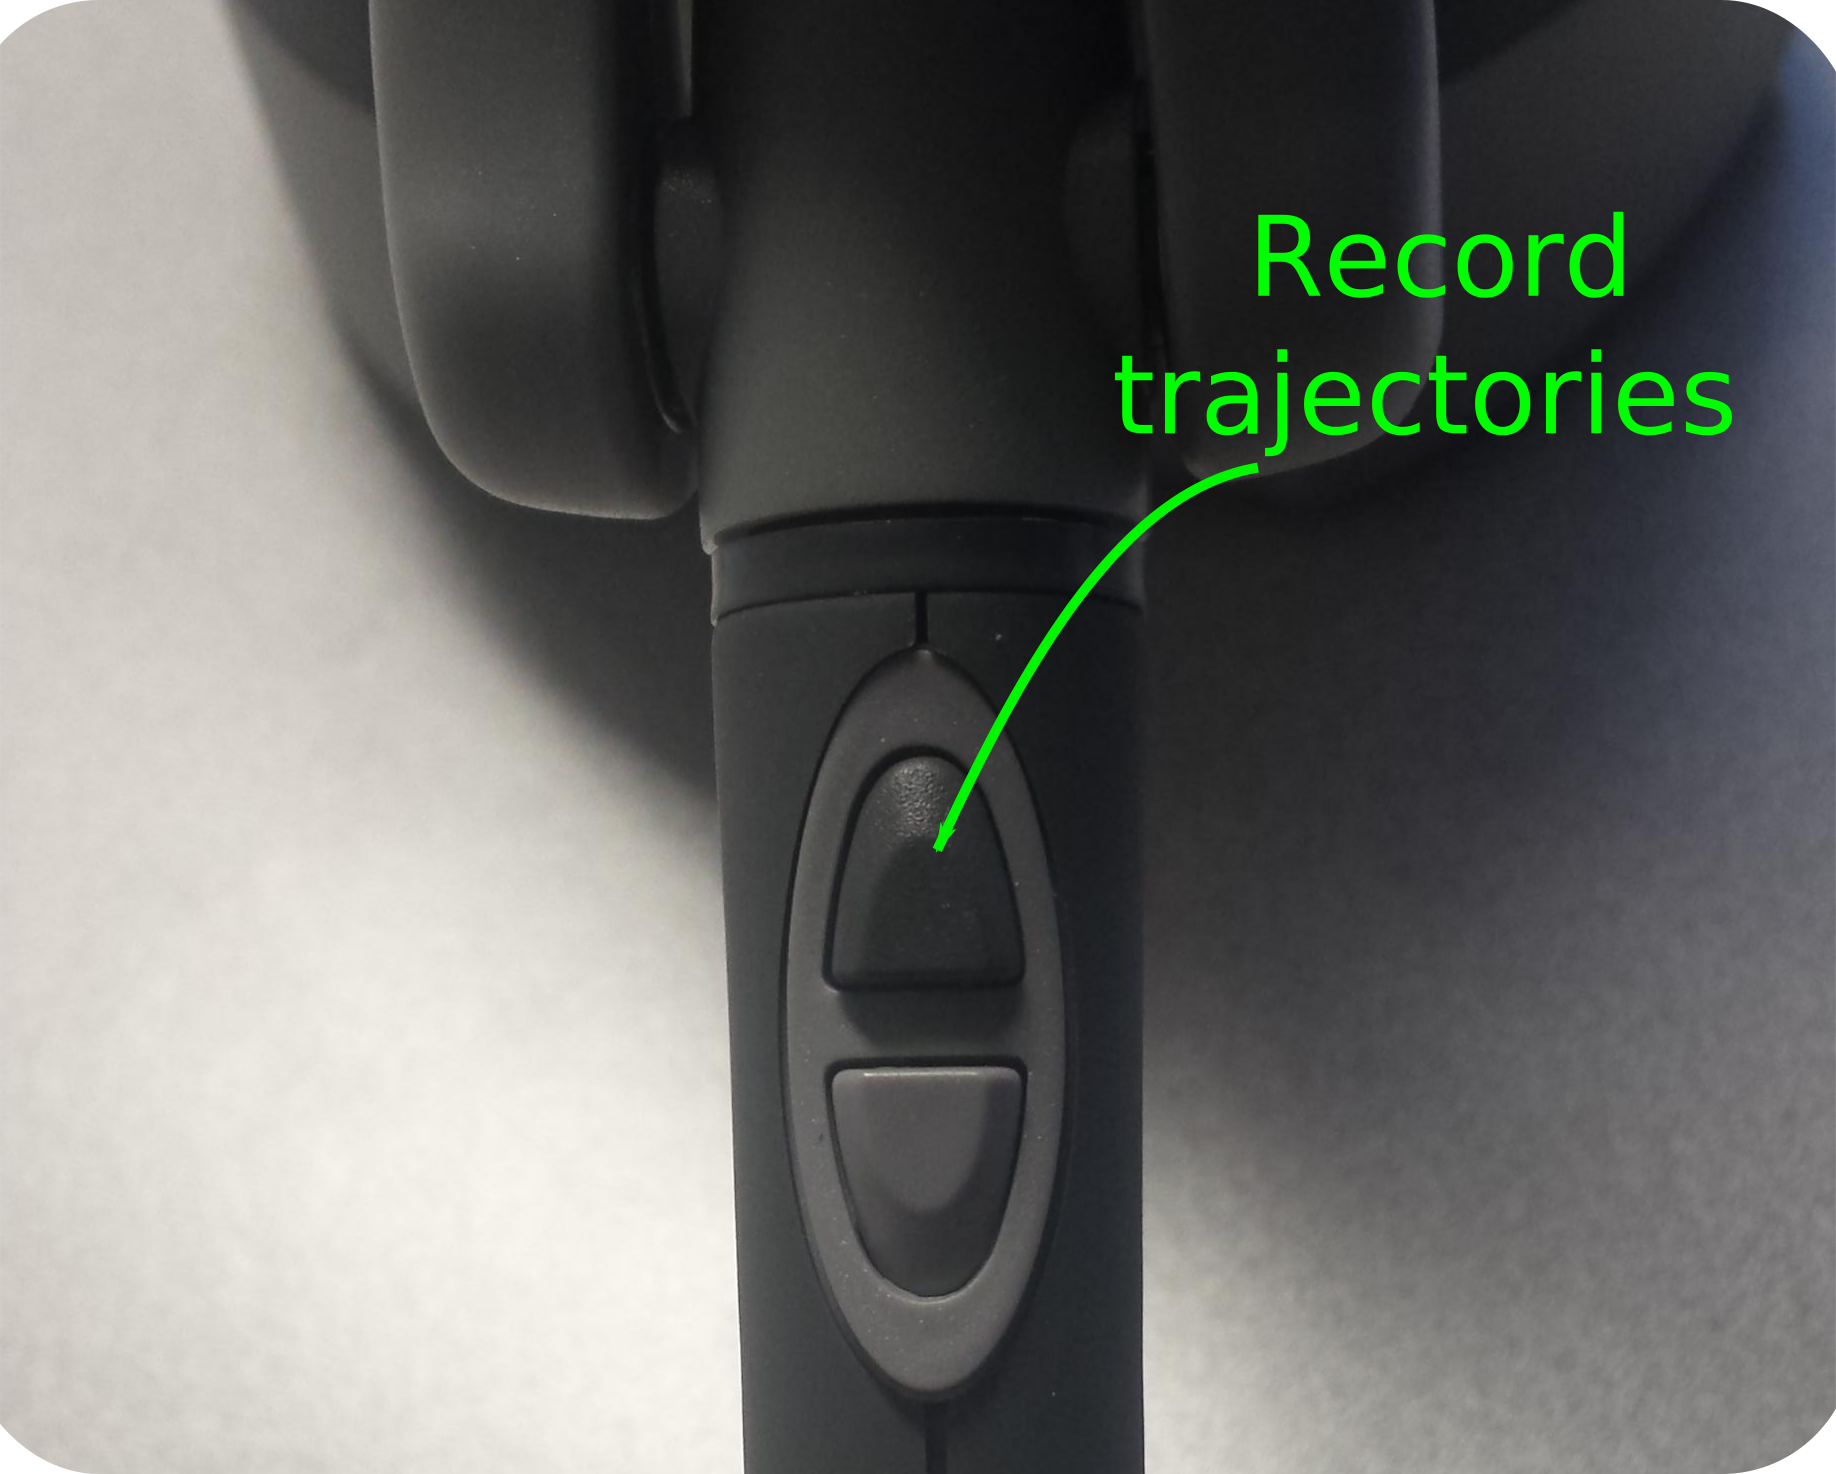
\includegraphics[height = 5cm]{img/geoButton.pdf}
%\caption{The dark button of the Geomagic.}
%\label{fig:geobuttons}
%\end{figure}

A video showing the iCub's arm moved by an user through the haptic device in Gazebo is available in Section~\ref{sec:video} (tutorial video).
The graph in Figure~\ref{fig:3TargetsTrajectories} represents some trajectories recorded with the Geomagic, corresponding to lifting the left arm of the iCub. % (in the iCub's frame).

%\begin{figure}[h]
%\centering
%\includegraphics[width=\hsize]{img/liftingWgeomagic/trajectory_sample.pdf}
%\caption{Some trajectories recorded when the Geomagic is used to lift the left arm: Cartesian position of the end-effector.}
%\label{fig:trajectories}
%\end{figure}

Demonstrated trajectories and their corresponding forces can be recorded directly from the robot, by accessing the Cartesian interface and the \textit{wholeBodyDynamicsTree} module.\footnote{\rev{In our example, we do not use the simulated wrench information as it is very noisy. However, we provide the code and show how to retrieve it and use it, in case the readers should not have access to the real iCub.}}

In our project on Github, we provide the acquired dataset with the trajectories for the interested reader who wishes to test the code with these trajectories. Two datasets are available at \url{https://github.com/inria-larsen/icubLearningTrajectories/tree/master/MatlabProgram/Data/}:  the first dataset called ``heights" is composed of three goal-directed reaching tasks, where the targets vary in height; the second dataset called ``FLT" is composed of trajectories recorded on the real robot, whose arms moves forward, to the left and to the top.

A matlab script that learns ProMPs with such kinds of datasets is available in the toolbox, called \mcode{demo_plotProMPs.m}. It contains all the following steps.

To load the first ``heights" dataset with the three trajectories, write:
\begin{lstlisting}
t{1} = loadTrajectory('Data/heights/bottom', 'bottom', 'refNb', s_bar, 'nbInput',nbInput, 'Specific', 'FromGeom');
t{2} = loadTrajectory('Data/heights/top', 'top', 'refNb', s_bar, 'nbInput',nbInput, 'Specific', 'FromGeom');
t{3} = loadTrajectory('Data/heights/middle', 'forward', 'refNb', s_bar, 'nbInput',nbInput, 'Specific', 'FromGeom');
\end{lstlisting}

Figure \ref{fig:3TargetsTrajectories} shows the three sets of demonstrated trajectories. In the used dataset called 	``heights", we have recorded $40$ trajectories per movement primitive.

%\begin{figure}[h]
%\centering
%{
%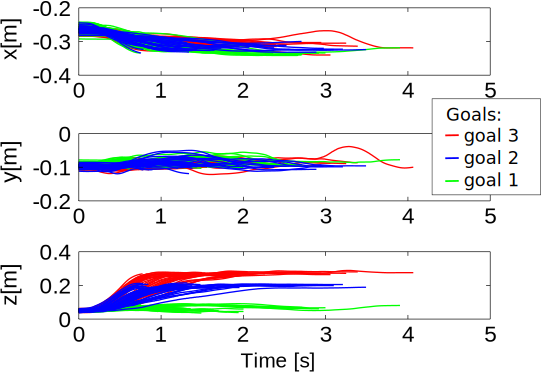
\includegraphics[width=12cm]{img/3DOFtrajectories.pdf}
%}
%\caption{Trajectories guided by the iCub's partner where he reaches three different positions that variate in height: in green the "bottom", in blue "middle" and in red "top goal positions. This plot represents only Cartesian position without force information.}% trajectories x (top),y(middle) and(bottom) without force information that are also recorded.}
%\label{fig:3TargetsTrajectories}
%\end{figure}

\subsection{Learning the ProMPs}


We need to first learn the ProMPs associated to the three observed movements. 
First, we partition the collected dataset into a training set and test dataset for the inference. One random trajectory for the inference is used:
%Before learning them, we pick from the training set one of the observed trajectory to test the inference, by writing for each $i$-th ProMP:
\begin{lstlisting}
[train{i},test{i}] = partitionTrajectory(t{i},1,percentData,s_bar);
\end{lstlisting}
The second input parameter specifies that we select only one trajectory, randomly selected, to test the ProMP. %With another number, for instance $10$, $10\%$ of the recorded data would be used for tests.

Now, we compute the three ProMPs with:

\begin{lstlisting}
promp{1} = computeDistribution(train{1}, M, s_bar,c,h);
promp{2} = computeDistribution(train{2}, M, s_bar,c,h);
promp{3} = computeDistribution(train{3}, M, s_bar,c,h)
\end{lstlisting}

We set the following parameters:
\begin{itemize}
\item \mcode{s\_bar=100}: reference number of samples, which we note in this paper as $\bar{s}$.
\item \mcode{nbInput(1) = 3; nbInput(2) = 6}: dimension of the generic vector containing the state of the trajectories. It is composed of 3D Cartesian position and 6D forces and wrench information.\footnote{Note that in our example wrenches are separated from the Cartesian position, because they are not used to recognize the index of the current ProMP during the inference.}
%\rev{dimension of the generic vector containing the state of the trajectories. It is composed of 3D Cartesian position and 6D forces and wrench information. Wrenches are separated from the Cartesian position, because they are not used to recognize the index of the current ProMP during the inference.}
\item \mcode{M(1) = 5; M(2)= 5}: number of basis functions for each \mcode{nbInput} dimension.
\item \mcode{c = 1/M;h = 1/(M*M)}: \textit{RBF} parameters (see Equation~\ref{eq:RBF}).
\item \mcode{expNoise = 0.00001}: the expected data noise. We assume this noise to be very low, since this is a simulation.
\item \mcode{percentData = 40}: this variable specifies the percentage of the trajectory that the robot will be observed, before infering the end.
\end{itemize}
These parameters can be changed at the beginning of the Matlab script.


Figure \ref{fig:3TargetsZTrajectoriesProMP} shows the three ProMPs of the reaching movements towards the three targets. To highlight the most useful dimension, we only plot the $z$-axis Cartesian position. However, each dimension is plotted by the Matlab script with:
\begin{lstlisting}
drawRecoverData(t{1}, inputName, 'Specolor','b','namFig', 1);
drawRecoverData(t{1}, inputName, 'Interval', [4 7 5 8 6 9], 'Specolor','b','namFig',2);
drawRecoverData(t{2}, inputName, 'Specolor','r','namFig',1);
drawRecoverData(t{2}, inputName, 'Interval', [4 7 5 8 6 9], 'Specolor','r','namFig',2);
drawRecoverData(t{3}, inputName, 'Specolor','g','namFig',1);
drawRecoverData(t{3}, inputName, 'Interval', [4 7 5 8 6 9], 'Specolor','g','namFig',2);
\end{lstlisting}

%We used the following parameters \todo{explain params...}

%\begin{figure}[h]
%\centering
%{
%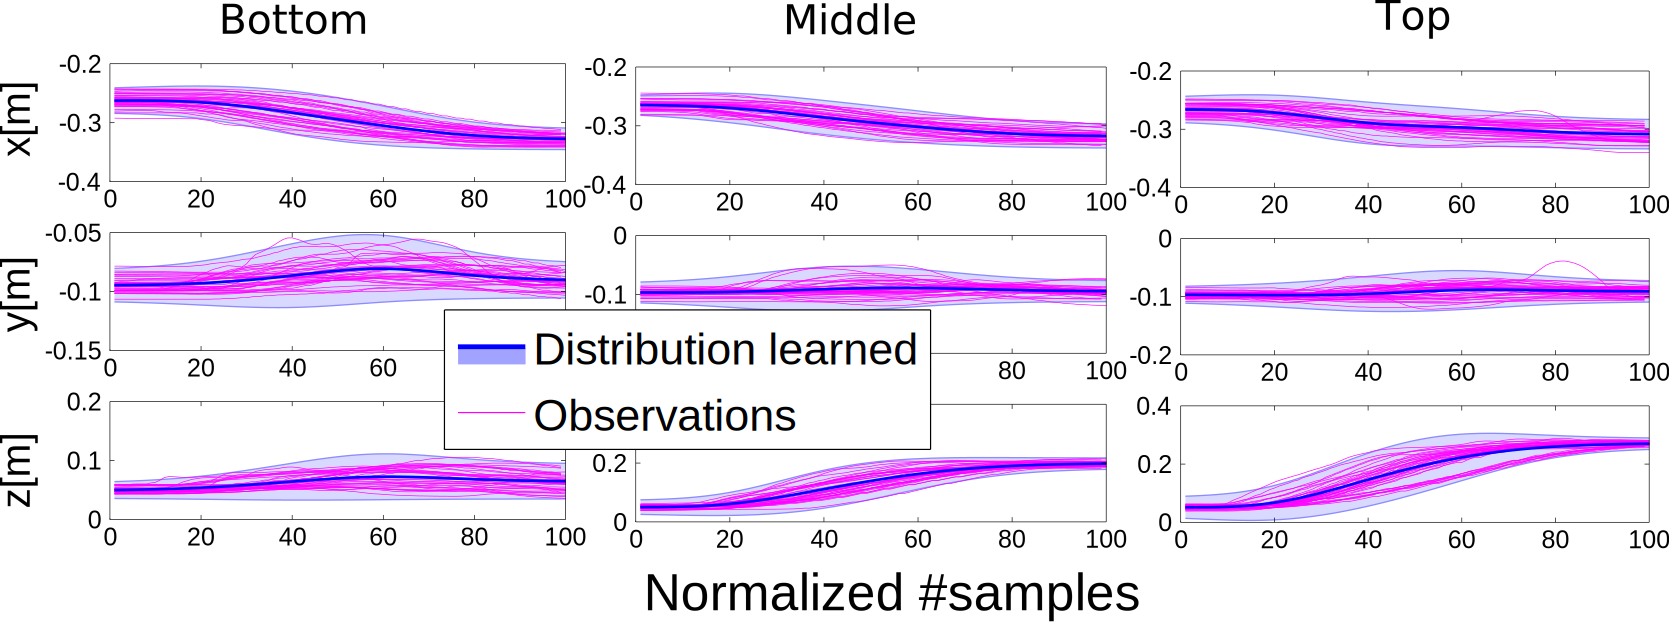
\includegraphics[width=\hsize]{img/3DOFtrajectoriesProMPsAll.pdf}\\
%}
%\caption{The ProMPs of the three different demonstrated tasks, from $39$ trajectory observations per ProMP; with M=5 basis functions per information learned; $c={1 \over M}, h={1 \over M^2}$ the parameters of the \textit{RBFs}' Gaussians, $\bar{s} = 100$ the reference number of samples. Note that we represent only the Cartesian position without force information to be readable.}
%\label{fig:3TargetsTrajectoriesProMP}
%\end{figure}
\begin{figure}[h]
\centering
{
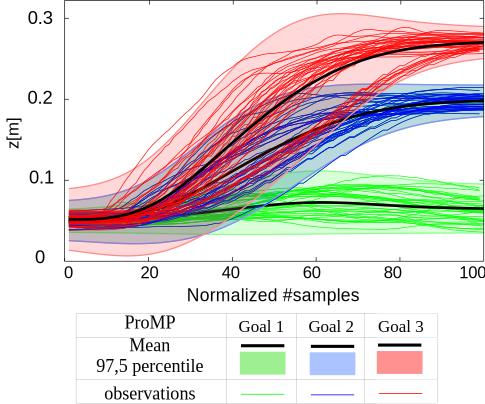
\includegraphics[height=8cm]{img/3DOFtrajectoriesProMPs.pdf}
}
\caption{The Cartesian position in the $z$-axis of the three ProMPs corresponding to reaching three targets. There are $39$ trajectory demonstrations per each ProMPm with M=5 basis functions, $c={1 \over M}, h={1 \over M^2}$ and $\bar{s} = 100$.}
\label{fig:3TargetsZTrajectoriesProMP}
\end{figure}


\subsection{Predicting the desired movement}

Now that we have learned the different ProMPs, we can predict the end of a trajectory according to the early observation $n_o$.
This number is computed from the variable \mcode{percentData} written at the beginning of the trajectory by: $n_o= |{percentData \over 100}* t_{fi}|$, where $i$ is the index of the test-trajectory

To prepare the prediction, the model the time modulation of each trajectory is computed with:
\begin{lstlisting}
    w = computeAlpha(test.nbData,t, nbInput);
    promp{1}.w_alpha= w{1};
    promp{2}.w_alpha= w{2};
    promp{3}.w_alpha= w{3};
\end{lstlisting}
This model relies on the global variation of Cartesian position during the first $n_o$ observations. The model's computations are explained in Section~\ref{sec:predictDuration}.

Now, to estimate the time modulation of the trajectory, call the function:
\begin{lstlisting}
[alphaTraj,type, x] = inferenceAlpha(promp,test{1},M,s_bar,c,h,test{1}.nbData, expNoise, 'MO');
\end{lstlisting}
Where \mcode{alphaTraj} contains the estimated time modulation $\hat{\alpha}$ and \mcode{type} gives the index of the recognized ProMP. The last parameter \mcode{x} is used for debbuging purposes.

% This variable vector contains the early observations of the trajectory translated with an offset to be centred at the mean of the recognized ProMP.  
%\marco{why the mean? Why this translation?}
%\rev{It is hard to explain in english for me, I join a picture to explain the idea}

Using this estimation of the time modulation, the end of the trajectory is inferred with:
\begin{lstlisting}
infTraj = inference(promp, test{1}, M, s_bar, c, h, test{1}.nbData, expNoise, alphaTraj);
\end{lstlisting}
%
%It can be interesting to plot the predicted trajectories for the different targets, after few or more observations. The Figure~\ref{fig:1DOFtrajectoriesPredictions3targets} represent such plots.

%\begin{figure}[!h]
%\centering
%{
%Target: green (bottom)
%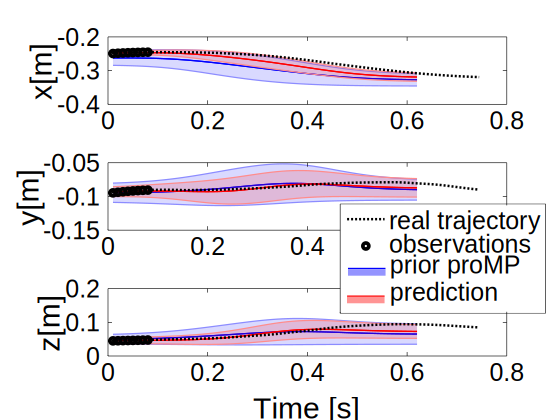
\includegraphics[width=\hsize /2]{img/infData3D/bottom10.pdf}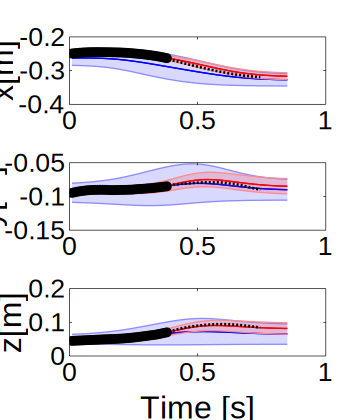
\includegraphics[width=\hsize /2]{img/infData3D/bottom50.pdf}
%%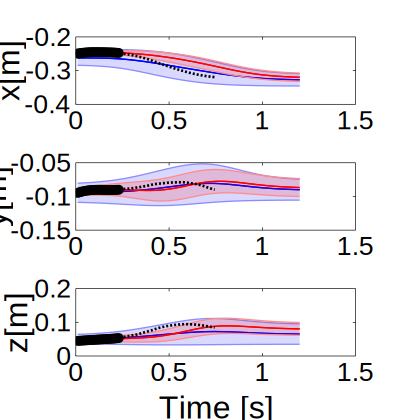
\includegraphics[width=\hsize /3]{img/infData3D/bottom30.pdf}
%Target: blue (middle)
%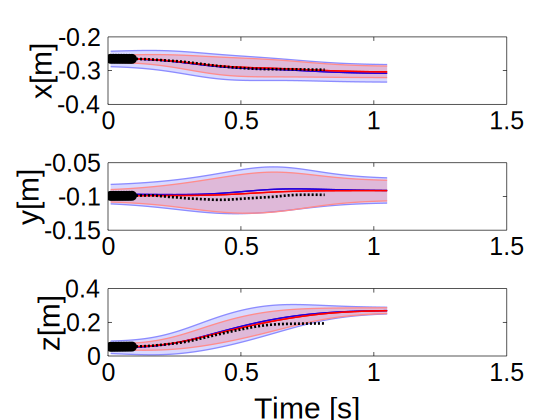
\includegraphics[width=\hsize /2]{img/infData3D/middle10Err.pdf}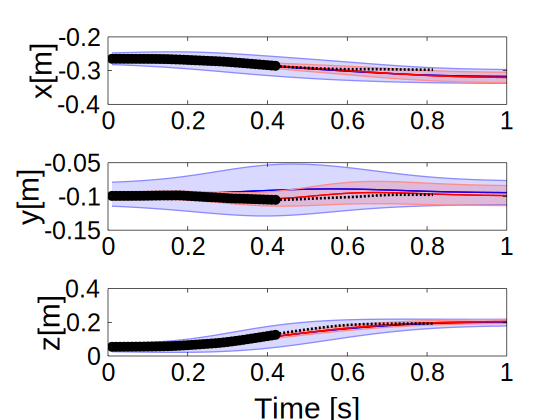
\includegraphics[width=\hsize /2]{img/infData3D/middle50.pdf}
%%%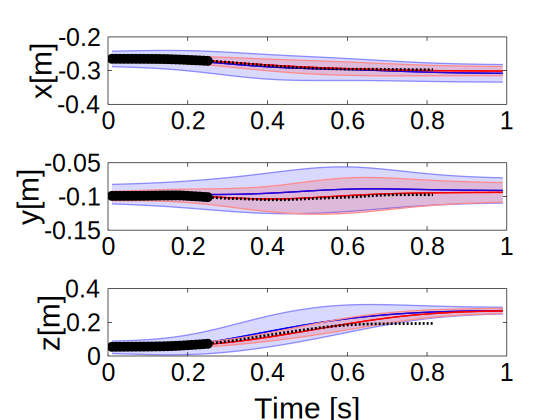
\includegraphics[width=\hsize /3]{img/infData3D/middle30Err.pdf}
%Target: red (top) 
%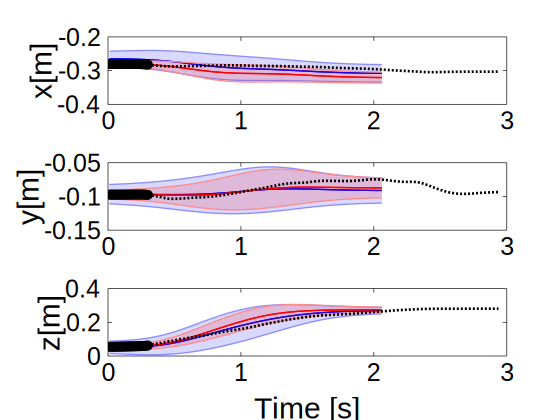
\includegraphics[width=\hsize /2]{img/infData3D/top10.pdf}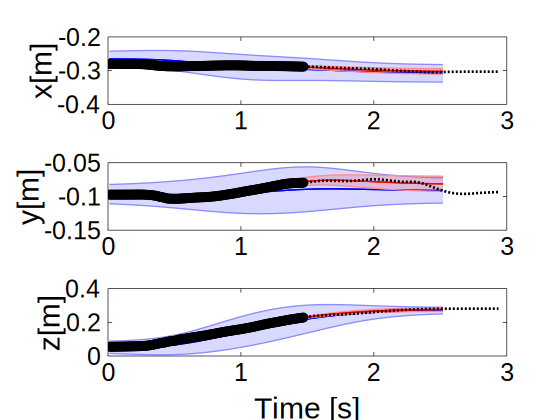
\includegraphics[width=\hsize /2]{img/infData3D/top50.pdf}
%%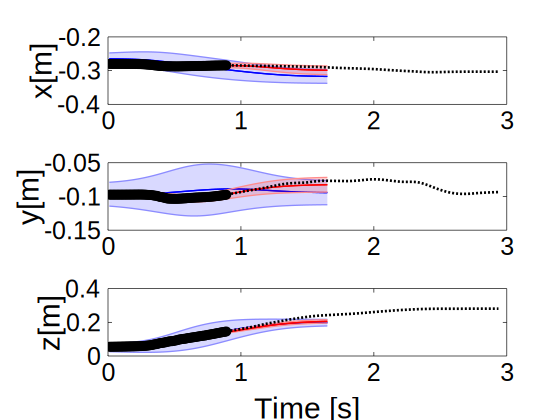
\includegraphics[width=\hsize /3]{img/infData3D/top30.pdf}
%}
%\caption{The prediction of the future trajectory thanks to the learned ProMPs computed for the  3-targets dataset (Figure \ref{fig:3TargetsZTrajectoriesProMP}) after 10 and 50 observations.}
%\label{fig:1DOFtrajectoriesPredictions3targets}
%\end{figure}

%\todo{l'image n'est pas clair, on ne voit pas grand chose : comment rendre ça plus clair ?}

As shown in the previous example, the quality of the prediction of the future trajectory depends on the accuracy of the time modulation estimation. This estimation is computed by calling the function: 
\begin{lstlisting}
%Using the model:
[alphaTraj,type, x] = inferenceAlpha(promp,test{1},M,s_bar,c,h,test{1}.nbData, expNoise, 'MO');
%Using the distance criteria:
[alphaTraj,type, x] = inferenceAlpha(promp,test{1},M,s_bar,c,h,test{1}.nbData, expNoise, 'DI');
%Using the Maximum likelihood criteria:
[alphaTraj,type, x] = inferenceAlpha(promp,test{1},M,s_bar,c,h,test{1}.nbData, expNoise, 'ML');
%Using the mean of observed temporal modulation during learning:
alphaTraj = (promp{1}.mu_alpha + promp{2}.mu_alpha + promp{3}.mu_alpha) /3.0;  
\end{lstlisting}

%% Sere: this figure seems not correct, we better remove it
%Figure \ref{fig:3DOFtrajectoriesPredictionsDuration} shows the trajectories predicted after $n_{o}=40$ observations of a desired trajectory, with or without the prediction of the trajectory duration. The last plot shows the baseline prediction, which uses the average duration extracted from the ProMP; the other plots show the prediction using (top-left) the model of the time modulation according to the global variation of position; (top-right) the maximum likelihood that the observed trajectory is assimilated to the ProMP, tested with each $\alpha$ observed during learning; the minimum distance between the observed trajectory and each ProMP rescaled with each $\alpha$ observed during the learning.
%\begin{figure}[h]
%\centering
%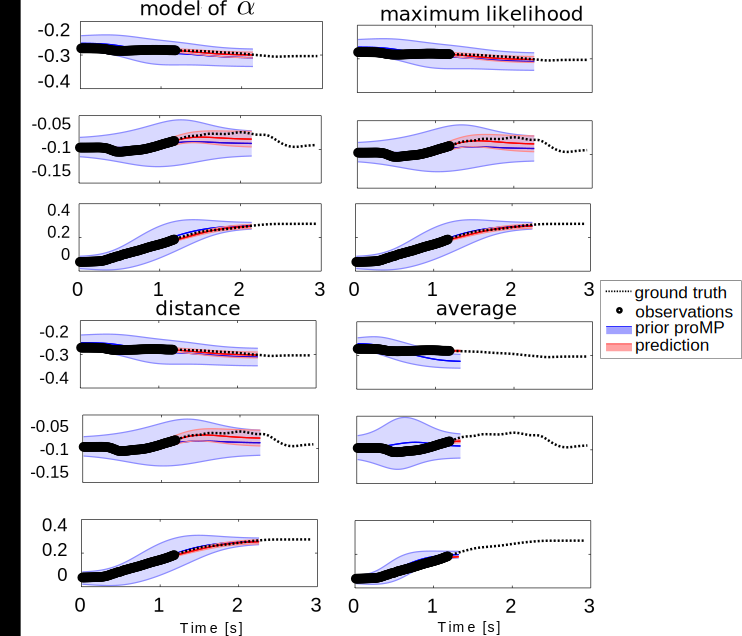
\includegraphics[height =  15cm]{img/3DOFtrajectoriesPredictionsDuration.pdf}
%\caption{The prediction of the future trajectory given $n_{o}=40$ early observations thanks to the learned ProMPs computed for the test dataset (Figure \ref{fig:3TargetsZTrajectoriesProMP}). The plots show the predicted trajectories: 1) using the model of $alpha$ according to the global position variation during the $n_o$ first observations; 2) using the maximum likelihood criteria 3) using the minimum distance criteria 4) using the average duration of the ProMP. Only one example for the red target is shown here.}
%\label{fig:3DOFtrajectoriesPredictionsDuration}
%\end{figure}

\subsection{Predicting the time modulation}\label{sec:simulatedTimeModulationModels}

In Section \ref{sec:predictDuration} we presented four main methods for estimating the time modulation parameter, discussing why this is crucial for a better estimation of the trajectory. 
Here, we compare the methods on the three goals experiment.
% consisting of learning three ProMPs where the final position varies in the height position ($z$-axis in Cartesian coordinates). 
We recorded 40 trajectories for each movement primitive, 
%executed by four different human participants, 
for a total of 120 trajectories.
%, with $40$ trajectories per each movement primitive. 
%This experiment has been done with four humans, that does ten trajectories for each movement primitive. Thus, we have forty observed trajectories per movements. 
After having computed the corresponding ProMPs, we tested the inference by providing early observations of a trajectory that the robot must finish. For that purpose, it recognizes the correct ProMP among the three precedently learned (see Section~\ref{sec:ManyProMP}) and then it estimates the time modulation parameter $\hat{\alpha}$.
%To understand how to infer a trajectory from many ProMPs, refer to Section~\ref{sec:ManyProMP}. 
Figure~\ref{fig:analyseAlpha} represents the average error of the $\hat{\alpha}$ during inference for 10 trials according to the number of observations (from 30\% to 90\% of observed data) and according to the used method. 
These methods are the ones we have just presented before that we called mean (Equation~\ref{eq:avg}), maximum likelihood (Equation~\ref{eq:ml}), minimum distance (Equation~\ref{eq:minDist}) or model (Equation~\ref{eq:model}). 
Each time, the tested trajectory is chosen randomly from the data set of observed trajectories (of course, the test trajectory does not belong to the training set, so it was not used in the learning step). 
\begin{figure}[h]
 \begin{minipage}[c]{.46\linewidth}
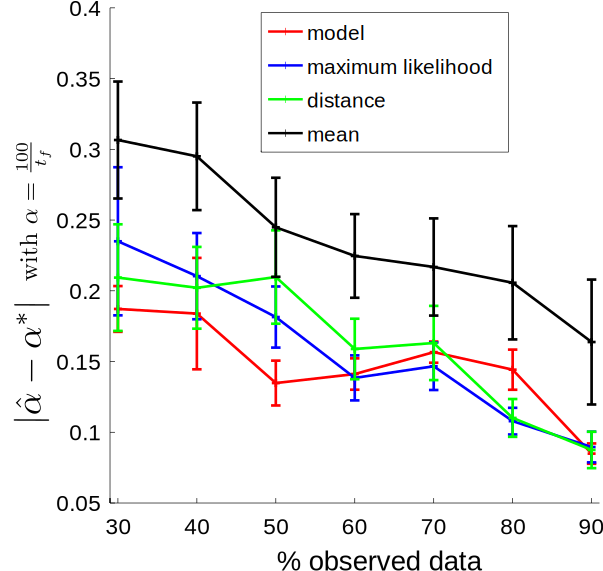
\includegraphics[width=\hsize]{img/alphaErrorAll.pdf}
\end{minipage} \hfill
   \begin{minipage}[c]{.46\linewidth}
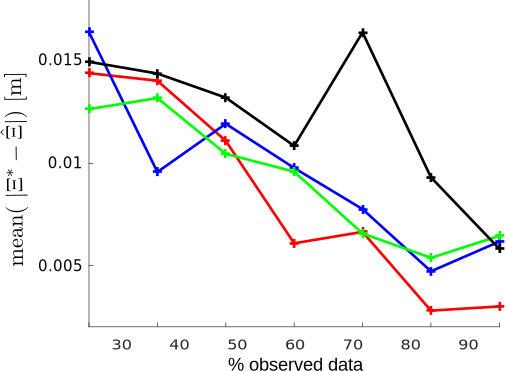
\includegraphics[width=\hsize]{img/YErrorAll.pdf}
\end{minipage}
\center
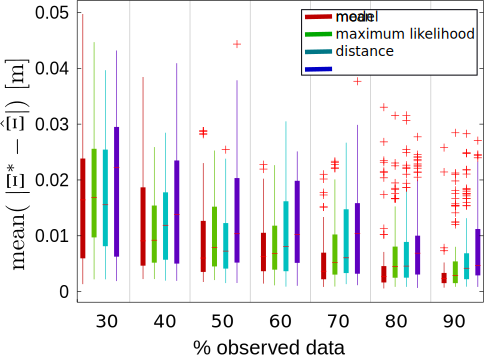
\includegraphics[height=6cm]{img/errorBoxplot.pdf}
\caption{(top left) Error of $\alpha$ estimation; (top right and bottom) error of trajectory prediction according to the number of known data and the method used. We executed 10 different trials for each case.}
\label{fig:analyseAlpha}
\end{figure}
The method that takes the average of $\alpha$ observed during learning is taken as comparison (in black). We can see that other methods are more accurate. \rev{The \textit{maximum likelihood} is increasingly more accurate, as expected. The fourth method (\textit{model}) that models the $\alpha$ according to the global variation of the trajectory's positions during the early observations is the best performing when the portion of observed trajectory is small (\textit{e.g.}, 30\%-50\%).  Since it is our interest to predict the future trajectory as early as possible, we adopted the \textit{model} method for our experiments.}
%Note that even though 



%\newpage
%%%%%%%%%%%%%%%%%%%%%%%%%%%%%%%%%%%%%%%%%%%%%%%%%%%%%%%%%%%%%%%%%%%%%%%%%%%%%%%%
\section{Application on the real iCub}
\label{sec:appliRealIcub}

\rev{In this section we present and discuss two experiments with the real robot iCub.}

\rev{In the first, we take inspiration from the experiment of the previous Section \ref{sec:3ProMPsAppli}, where the ``tasks'' are exemplified by simple point-to-point trajectories demonstrated by a human tutor. In this experiment we explore how to use wrench information and use known demonstrations as ground truth, to evaluate the quality of our prediction.}
%The task consists in collaborating with a human operator to sort objects. 

%As an example, imagine a classic object sorting scenario, where the tasks could be transferring the objects to the correct bin or tray, or an assembly scenario where the tasks are different object-picking and manipulation trajectories, to be performed with or without the human partner.
%}

\rev{In the second experiment, we set up a more realistic collaborative scenario, inspired by collaborative object sorting. 
In such applications, the robot is used to lift an object (heavy, or dangerous, or that the human cannot manipulate, as for some chemicals or food), the human inspects the object and then decides if it is accepted or rejected. Depending on this decision, the object goes on a tray or bin in front of the robot, or on a bin located on the robot side. 
Dropping the objects in two cases must be done in a different way. Realizing this application with iCub is not easy, as iCub cannot lift heavy objects and has a limited workspace. Therefore, we simplify the experiment with small objects and two bins. The human simply starts the robots movement with physical guidance, and then the robot finishes the movement on its own.
In this experiment the predicted trajectories are validated on-the-fly by the human operator.}

\rev{In a more complex collaborative scenario, tasks could be elementary tasks such as pointing, grasping, reaching, manipulating tools (the type of task here is not important, as long as it can be represented by a trajectory).}


\subsection{Three simple actions with wrench information}

\rev{Task trajectories, in this example, have both position and wrench information.
In general, it is a good idea to represent collaborative motion primitives in terms of both position and wrenches, as this representation enables using them in the context of physical interaction.
 Contrarily to the simulated experiment, here the inferred wrenches $\hat{F}_t$ correspond to the wrenches the robot should perceive if the partner was manually guiding the robot to perform the entire movement: indeed, these wrenches are computed from the demonstrations used to learn the primitive. 
The predicted wrenches can be used in different ways, depending on the application.
For example, if the partner breaks the contact with the robot, the perceived wrenches will be different. If the robot is not equipped with tactile or contact sensors, this information can be used by the robot to ``perceive'' the contact breaking and interpret it, for example, as the sign that the human wants the robot to continue the task on its own. 
Another use for the demonstrated wrenches is for detecting abnormal forces while the robot is moving: this use can have different applications, from adapting the motion to new environment to automatically detecting new demonstrations. 
Here, they are simply used to detect when the partner breaks the contact with the robot, and the latter must continue the movement on its own.
%In the current case where the partner let go of the robot, the forces will be weaker. Thus, in future work, if wrenches are stronger that the inferred forces, the robot will stop its action and follow the partner's guidance.
}

\rev{In the following, we present how to realize the experiment for predicting the user intention with the real iCub, using our software.}
%We tested our software on the real iCub. 
The robot must learn three task trajectories represented in Figure \ref{fig:realAppli}. In red, the first trajectory goes from an initial position \rev{in front of the robot} to its left (\rev{task} A). In \rev{green}, the second trajectory goes from the same initial position to the top (\rev{task C}). In \rev{blue}, the last trajectory goes from the top \rev{position to the position on the left (task B).}

\rev{To provide the demonstrations for the tasks, the human tutor used three visual targets shown on the iCub\_GUI, a basic module of the iCub code that provides a real-time synthetic and augmented view of the robot status, with arrows for the external forces and colored objects for the targets. 
One difficulty for novice users of iCub is to be able to drive the robot's arm making it perform desired complex 3D trajectories \cite{ivaldi2017towards}, but after some practice in moving the robot's arm the operator recorded all the demonstrations.
We want to highlight that having variations in the starting or ending points of the trajectories is not at all a problem, since the ProMPs are able to deal with this variability.%, contrarily to other methods for synthesizing motion primitives.
}


%One challenge of this real-world application is that the robot's arm is not easy to handle. The user need to control all the robot's degrees of freedom with one of his hands. Moreover, the user can guide the robot in different ways, so  there is variability in movements that reach the same goal.

%Despite these difficulties, we will see that 
We will see that by using the ProMPs method and by learning the end-effector Cartesian position, the robot will be able to learn distributions over trajectories, recognize when a movement belongs to one of these distributions and infer the end of the movement.


\begin{figure}[h]
\centering
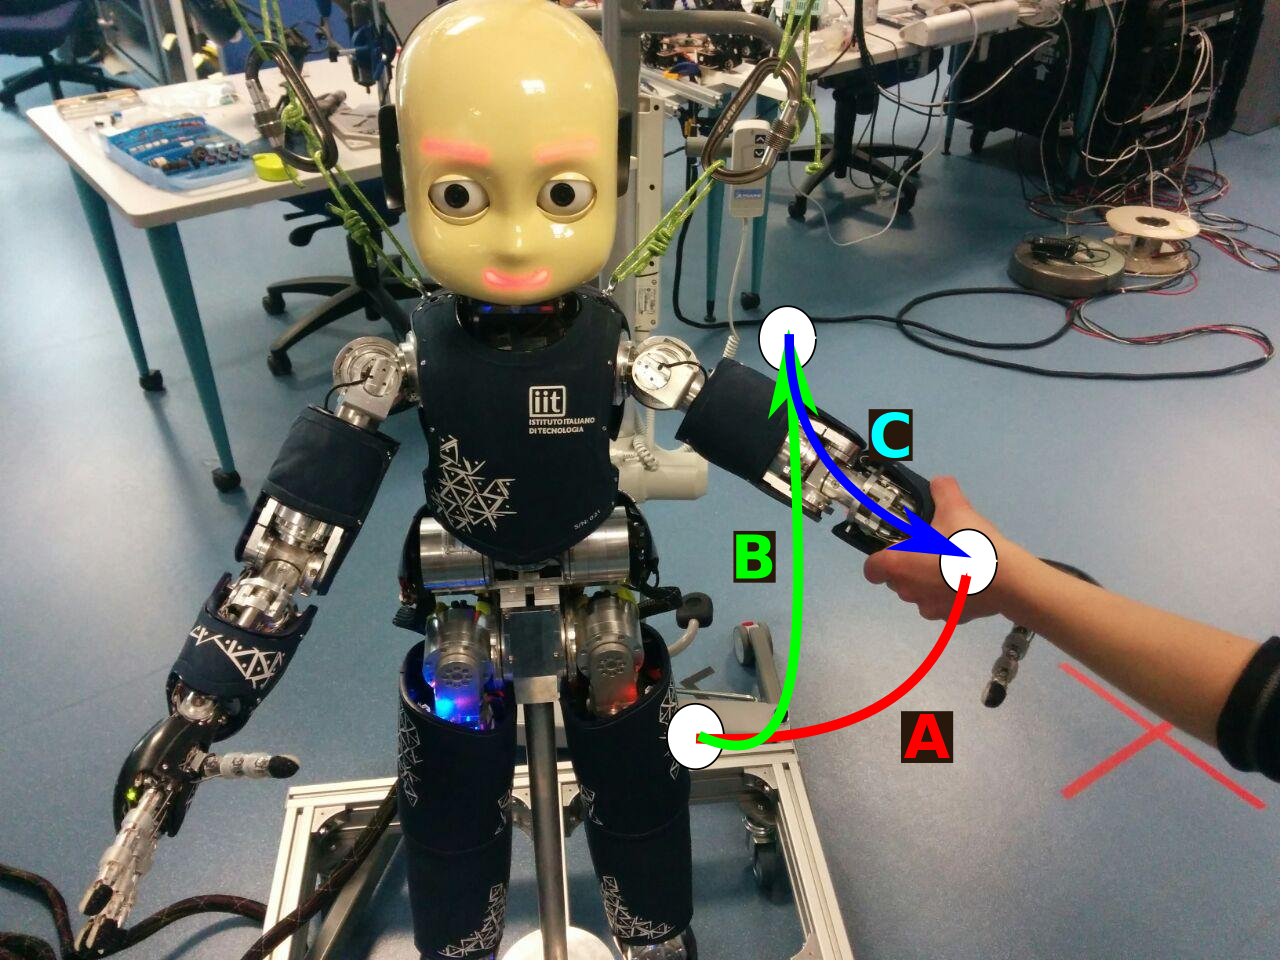
\includegraphics[width=9cm]{img/experimentRepresentation.pdf}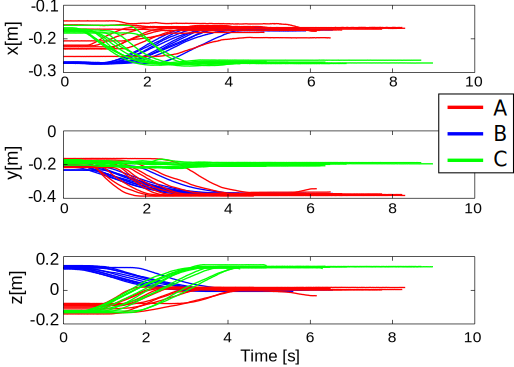
\includegraphics[width=10cm]{img/realTrajectories2.pdf}\\
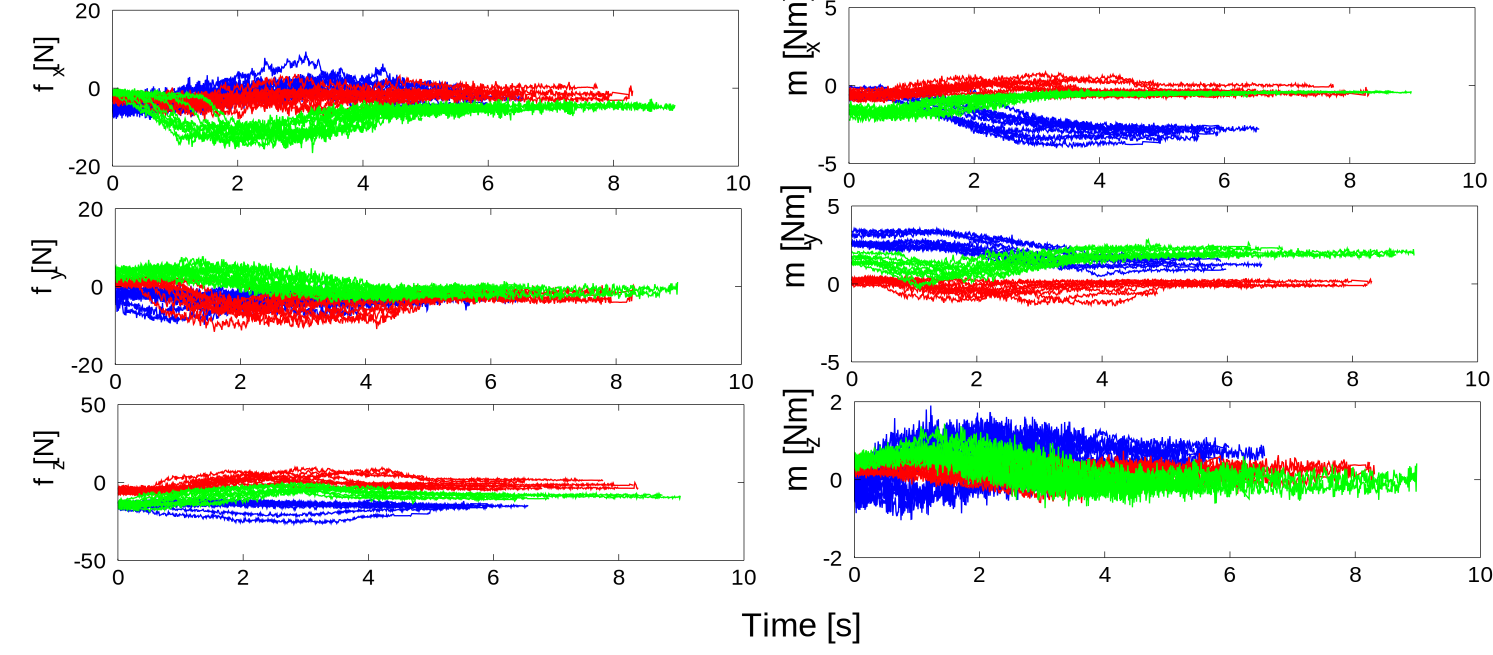
\includegraphics[width=18cm]{img/realTrajectoriesv2.pdf}
\caption{Top left: the iCub and the visualization of the three targets in its workspace, defining the three tasks A-B-C. Top right: Cartesian position information of the demonstrated trajectories for the three tasks. Bottom left and right: wrench (force and moment) information of the demonstrated trajectories.
%The three trajectories presenting the primitives A, B, and C. A color code (RGB) is used throughout the paper to facilitate the recognition of trajectories (top-left); and the corresponding test-set composed of position (top) and wrench (bottom) information.
}
\label{fig:realAppli}
\end{figure}

In this experiment, the robot received $10$ demonstrated trajectories per movement primitive, all provided by the same user. We recorded the Cartesian end-effector position and the wrenches of the robot's left arm. Data are retrieved using the function \mcode{used_functions/retrieveRealDataWithoutOrientation.m}. The output parameters of this function are three objects (one per ProMP) that contain all the required information to learn the ProMPs. 
%%From these objects, the robot learned:
%Each trajectory is:
%$$\Xi_t = \begin{bmatrix}
%[x_t & y_t & z_t ]^\top \\ [F_x & F_y & F_z]^\top \\ [m_x & m_y & m_z]^\top
%\end{bmatrix}$$
%\marco{[Obs.: What did the robot learn? The parameters $\omega$ and the distributions or the trajectories?]}
%\rev{I don't understand your question: by learning the $\omega$ parameter and the distributions, the robot learns the trajectory, isn't it?} 

In this function, the wrench information are filtered using a Matlab function called \mcode{envelope.m}\footnote{Information about this function can be found here: \url{https://fr.mathworks.com/help/signal/ref/envelope.html?requestedDomain=www.mathworks.com}}: for each trajectory \mcode{traj} and its subMatrix $M = F([1:t])$:
\begin{lstlisting}
[envHigh, envLow] = envelope(traj.M);
traj.M = (envHigh+envLow)/2;
\end{lstlisting}
These three objects are saved in \mcode{'Data/realIcub.mat'}. A Matlab script called \mcode{demo_plotProMPsIcub.m} recovers these data, using the function \mcode{load('Data/realIcub.mat')}. This script follows the same organization as the ones we previously explained in Sections~\ref{sec:example1DOF} and \ref{sec:3ProMPsAppli}. 
By launching this script, the recovered data are plotted first.

%\begin{figure}[h]
%\centering
%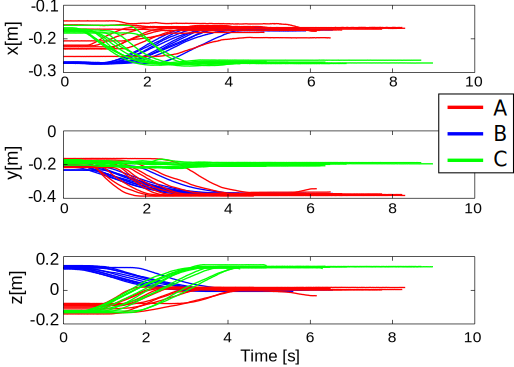
\includegraphics[height = 10cm]{img/realTrajectories2.pdf} 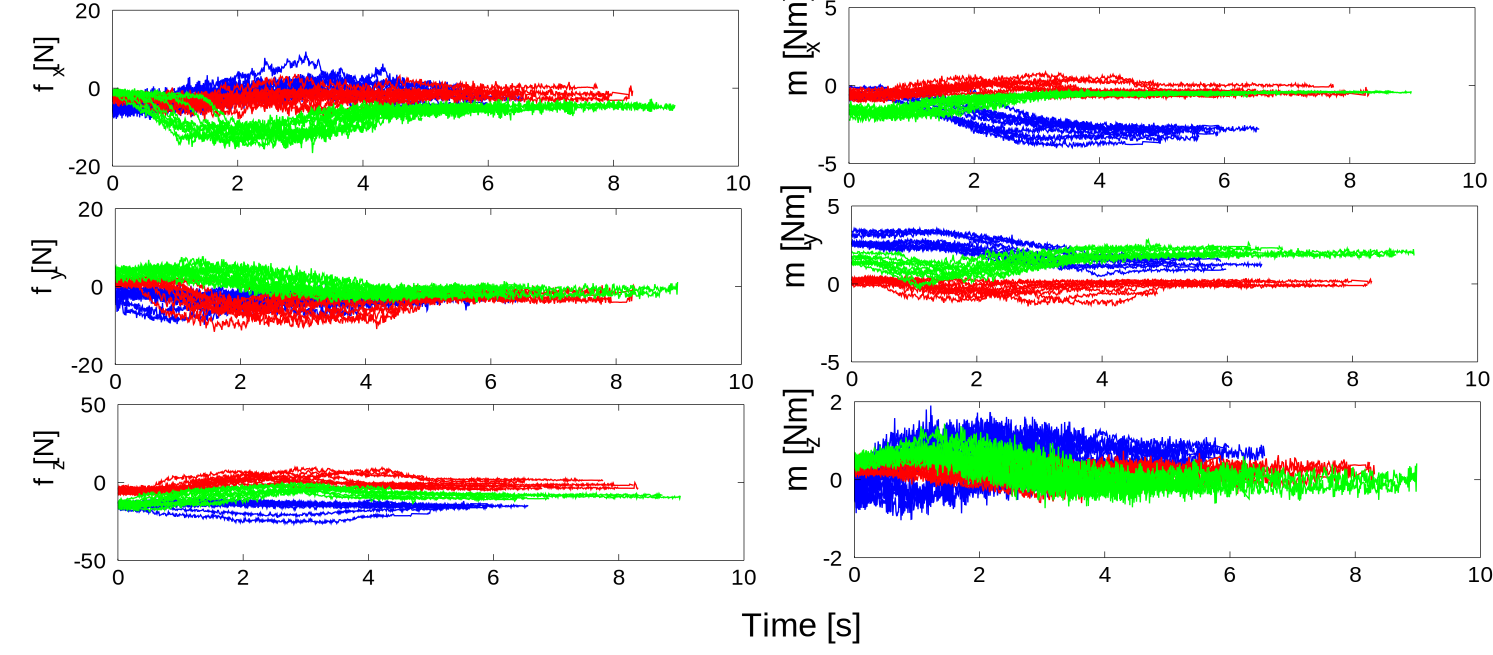
\includegraphics[width=\hsize]{img/realTrajectoriesv2.pdf} 
%\caption{Reprensentation of the three trajectories learned by the real iCub. Top: 3D Cartesian position; bottom: wrenches with 3D forces (left) and 3D moments (right).}
%\label{fig:realTraj}
%\end{figure}

Then, the ProMPs are computed and plotted, as presented in Figure~\ref{fig:realDistribution}.
In this figure, the distributions are visibly overlaid:
\begin{itemize}
\item during the whole trajectories duration for the wrench information;
% $f_x$, $f_y$, $f_z$ and $m_z$ dimensions; 
\item during the $40\%$ first samples of the trajectories for the Cartesian position information.
%$x$, $y$ and $z$ dimensions. 
\end{itemize}


%We make the hypothesis that force information is not useful for identifying trajectories. However, the robot learned it to know what are the forces' amplitude it is supposed to measure.




After this learning step, the user chooses which ProMP to test.
Using a variable that represents the percentage of observed data to be used for the inference, the script computes the number of early observations $n_o$\footnote{$n_o$ is not the same for each trajectory test, because it depends on the total duration of the trajectory to be inferred. } that will be measured by the robot. Using this number, the robot models the time modulation parameter $\alpha$\footnote{Since the model uses the $n_o$ parameter, its computation cannot be performed before this step.} of each ProMP, as explained in Section~\ref{sec:predictDuration}. 
Using this model, the time modulation of the test trajectory is estimated and the corresponding ProMP is identified.

%\begin{figure}[h]
%\centering
%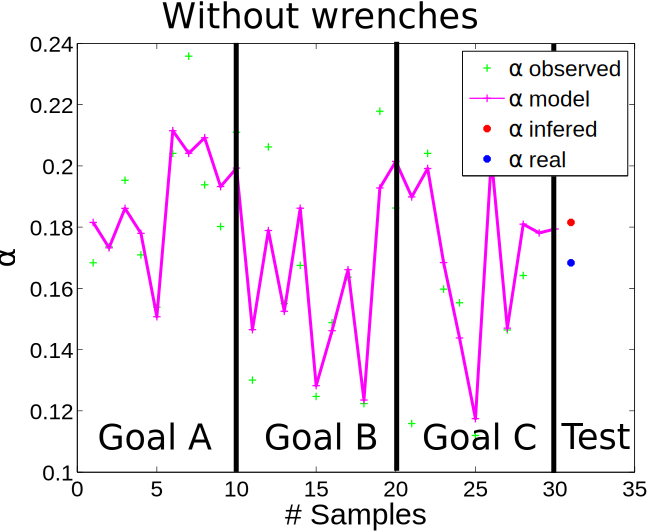
\includegraphics[width = 8cm]{img/realalphaModel.pdf} 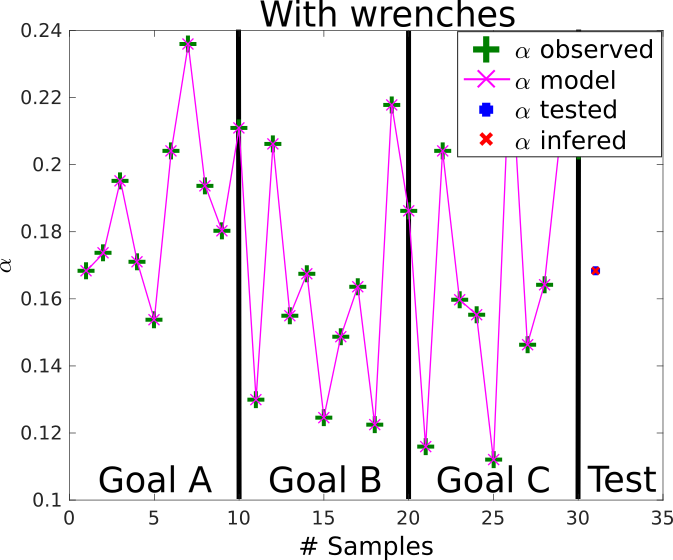
\includegraphics[width = 8cm]{img/alphaInfWithForces.pdf} 
%\caption{$\alpha$ model with (left) and without (right) wrenches. In pink, the $\alpha$ model based on the $\alpha$ set of the learning trajectories; in green, their real values; in red, the $\hat{\alpha}$ expectation of the test trajecory; and in blue its real value.
%}
%\label{fig:realalphaModel}
%\end{figure}

%Figure \ref{fig:realalphaModel} represents some $\alpha$ estimation using the learned model. On the left when the model doesn't contain wrench information, on the right with wrench information. The green crosses represent the $\alpha$ set of the learning trajectories, and the pink crosses the estimation done by the model based on this set. The $10$ first crosses are the $\alpha$ set of the first ProMP, the $10$ following the ones of the second ProMP and the last $10$ crosses the ones for the third ProMP. Finally, the red cross is the $\hat{\alpha}$ estimation of the test trajectory and the blue cross the real $\alpha$ of this test trajectory. We can see that with wrench information, the $\alpha$ estimation is really accurate.

\begin{figure}[!h]
\centering
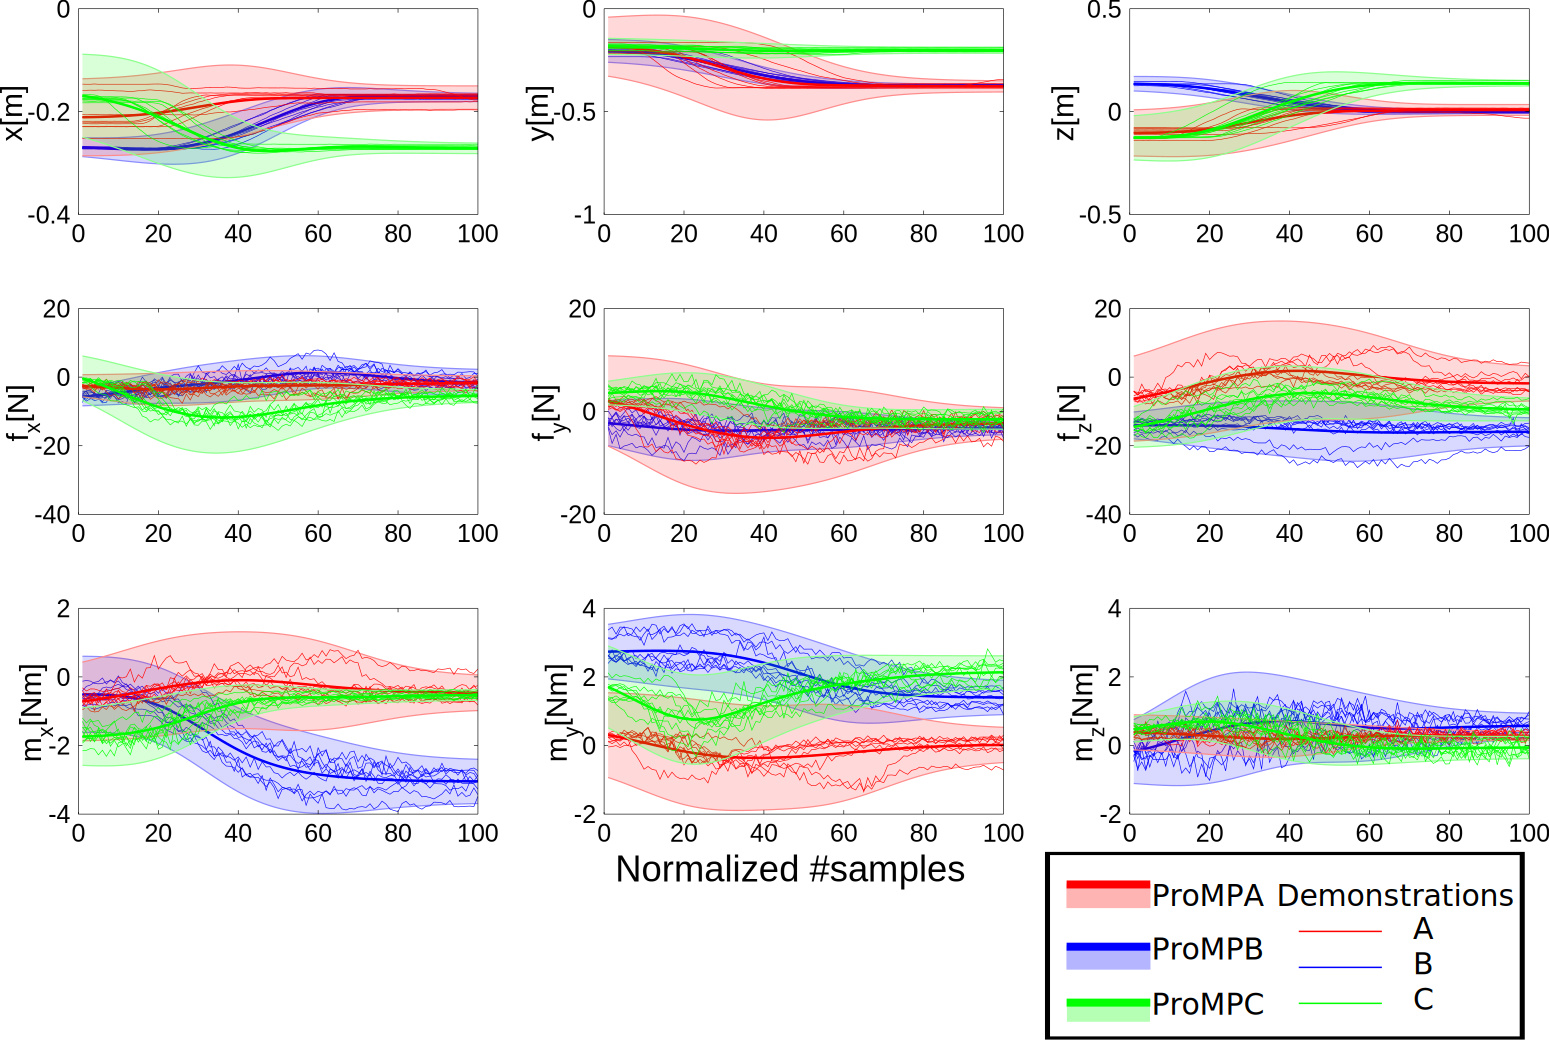
\includegraphics[height = 10cm]{img/realDistribution.pdf} 
\caption{The ProMPs learned by the robot from the demonstrations of Figure \ref{fig:realAppli}.}
\label{fig:realDistribution}
\end{figure}

\begin{figure}[!h]
\centering
{
\textcolor{red}{A}\\
\includegraphics[width=15cm]{img/infA.pdf}\\
%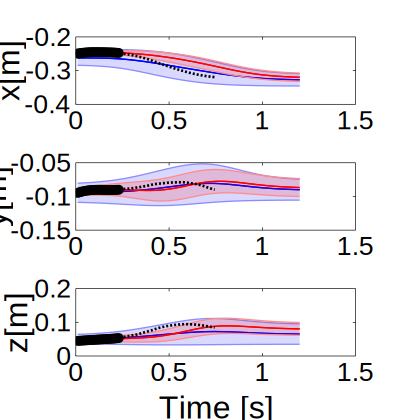
\includegraphics[width=\hsize /3]{img/infData3D/bottom30.pdf}
\textcolor{blue}{B}\\
\includegraphics[width=15cm]{img/infb.pdf}\\
%%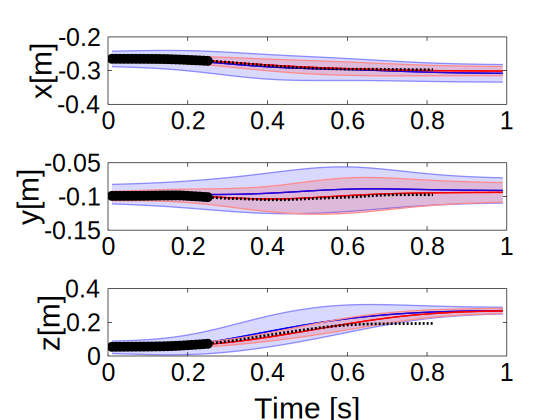
\includegraphics[width=\hsize /3]{img/infData3D/middle30Err.pdf}
\textcolor{green}{C}\\
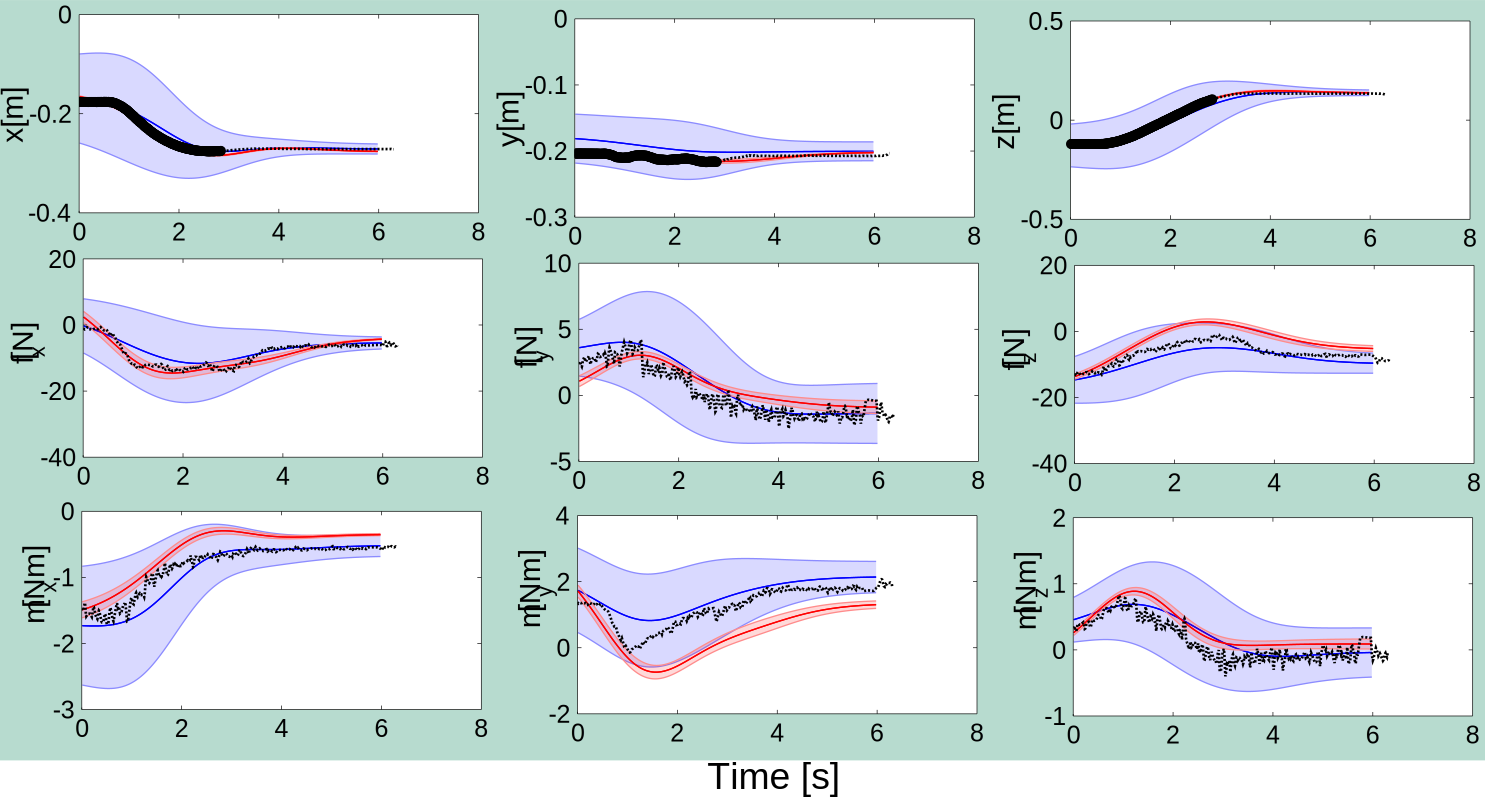
\includegraphics[width=15cm]{img/infc.pdf}\\
%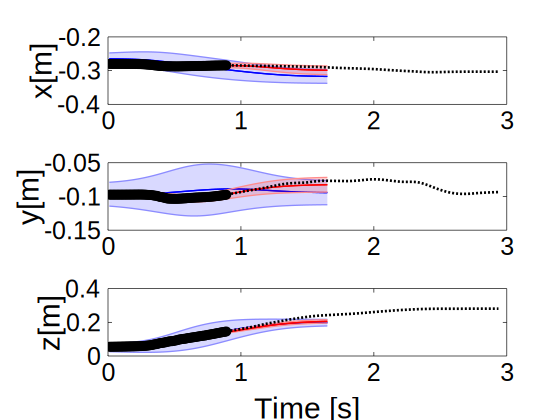
\includegraphics[width=\hsize /3]{img/infData3D/top30.pdf}
}
\caption{The prediction of the future trajectory from the learned ProMPs computed from the position information for the  3-targets dataset on the real iCub (Figure \ref{fig:realDistribution}) after 40\% of observations.}
\label{fig:realTrajectoriesPredictions}
\end{figure}

Then, the inference of the trajectory's target is performed. 
Figure~\ref{fig:realTrajectoriesPredictions} represents the inference of the three tested trajectories when wrench information is not used by the robot to infer the trajectory. 
\rev{To realize this figure, with the comparison between the predicted trajectory and the ground truth, we applied our algorithm offline. In fact, it is not possible at time $t$ to have the ground truth of the trajectory intended by the human from $t+1$ to $t_f$: even if we would tell to the human in advance the goal that he/she must reach for, the trajectory to reach that goal could vary. So, for the purpose of these figures and comparisons with the ground truth, we show here the offline evaluation: we select one demonstrated task trajectory from the test set (not the training set used to learn the ProMP) as ground truth, and imagine that this is the intended trajectory.
In Figure~\ref{fig:realTrajectoriesPredictions}, the ground truth is shown in black, whereas the portion of this trajectory that is fed to the inference, and that corresponds to the ``early observations'', is represented with bigger black circles.
}
%\rev{These tests have been done on a test base, that contains some whole-trajectories guided by the user. Then, we give to the program only a partial trajectory composed on 40\% of the recorded trajectory. The ground truth (\textit{e.g.} the total-trajectories of the test base) are represented in the figure in black. The partial-trajectories, that are known by the software are represented with the black circles.} 
We can see that the inference of the Cartesian position is correct, although we can see an error of about $1$ second of the estimated duration time for the last trial. Also, the wrench inference is not accurate. We can assume that it is: because the robot infers the trajectory using only position information without wrench information, or because the wrenches' variation is not correlated to the position variation.
To improve this result, we can make the inference using wrench in addition to Cartesian position information, as shown in Figure~\ref{fig:realTrajectoriesPredictionsWithForces}. We can see in this Figure that the estimation of the trajectory's duration is accurate. The disavantage is that the inference of the Cartesian position is less accurate because the posterior distribution computation makes a trade-off between fitting Cartesian position and wrench early observations. Moreover, to allow a correct inference using wrench information, the noise expectation must be increased to consider forces. \footnote{In future versions, we will include the possibility to have different noise models for the observations, \textit{e.g.} we will have $\Sigma_\Xi^o = \left[
\begin{array}{c c}
\Sigma_X  & 0\\  
0 &\Sigma_F \\
\end{array}\right]$. We will therefore set a bigger covariance for the wrench information than for the position information.}


%allow to have different expectation noises according to the data type
%\textcolor{blue}{expectation noises [Obs.: Is “noise
%expectation” or “expectation noise” the same as “observation noise”?]}
%\textcolor{purple}{@marco: i didn't understand your question but tell me if it is more clear now with the following parenthesis} 


To confirm these results, we analyzed the trajectory inference and $\alpha$ estimation considering different percentages of each trajectory as observed data ($30$ to $90\%$). For each percentage, we performed $20$ tests, with and without force information.


In Figure~\ref{fig:errBoxWithWithoutForces}, each box-plot represents errors for $20$ tests.
On the top, the error criterion is the average distance between the inferred trajectory and the real one. We can see that the inference of Cartesian end-effector trajectory is more accurate without wrench information.
On the bottom, the error criterion is the distance between the estimated $\alpha$ and the real one. We can see that using wrench information, the estimation of the $\alpha$ is more accurate.
Thus, these two graphs confirm what we assumed from Figures~\ref{fig:realTrajectoriesPredictions} and ~\ref{fig:realTrajectoriesPredictionsWithForces}. 

\rev{Median, mean and variance of the prediction errors, computed with the normalized root-mean-square error (NRMSE) are reported in Table~\ref{table:statsError}. 
The prediction error for the time modulation is a scalar: $|\alpha_{\textrm{prediction}} - \alpha_{\textrm{real}} |$.   
The prediction error for the trajectory is computed by the NRMSE of $| \Xi_{\textrm{prediction}} - \Xi_{\textrm{real}}  |$.}

In future upgrades for this application, we will probably use the wrench information only to estimate the time modulation parameter $\alpha$, to have both the best inference of the intended trajectory and the best estimation of the time modulation parameter to combine the benefits of inference with and without wrench information.


\rev{
Table~\ref{table:statsError} also reports the average time for computing the prediction of both time modulation and posterior distribution.  The computation were performed in Matlab, on a single core laptop (no parallelization). While the computation time for the case ``without wrenches'' is fine for real-time application, using the wrench information delays the prediction and represents a limit for real-time applications if fast decisions have to taken by the robot. Computation time will be improved in the future works, with the implementation of the prediction in an iterative way.
}

%or change the tolerance interval of accepted wrenches \todo{as represented in figure\ref{}}.

\begin{figure}[!h]
\centering
{
\textcolor{red}{A}\\
\includegraphics[width=14cm]{img/withWrenchInfA.pdf}\\
\textcolor{blue}{B}\\
\includegraphics[width=14cm]{img/withWrenchInfB.pdf}\\
\textcolor{green}{C}\\
\includegraphics[width=14cm]{img/withWrenchInfC.pdf}\\
%\includegraphics[height=20cm]{img/infUseForces.pdf}
}
\caption{The prediction of the future trajectory from the learned ProMPs computed from the position and wrench information for the 3-targets dataset on the real iCub (Figure \ref{fig:realDistribution}) after 40\% of observations.}
\label{fig:realTrajectoriesPredictionsWithForces}
\end{figure}


\begin{figure}[!h]
\centering
{
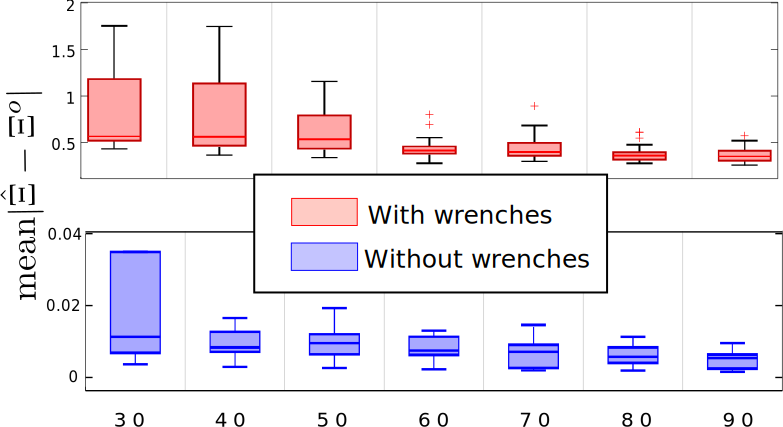
\includegraphics[width=12cm]{img/errBoxWithWithoutForces.pdf}\\
\includegraphics[width=12cm]{img/boxAlphaErrorWithForces.pdf}
}
\caption{Trajectory prediction error (top) and time modulation estimation error (bottom) of the future trajectory with and without wrench information, for the 3-targets dataset on the real iCub (Figure \ref{fig:realDistribution}) with respect to the number of observed data points.}
\label{fig:errBoxWithWithoutForces}
\end{figure}

%\begin{table}
%\centering
%\begin{tabular}{|c|c|c|c|c|c|c|c|}
% \hline
% Percentage of observations & 30 & 40 & 50 & 60 & 70 & 80 & 90 \\
% \hline
% Trajectory prediction error &   &    &    &    &    &    &    \\
% \hline
% Time modulation prediction error & & & & & & & \\
% \hline
% Computation time for prediction & & & & & & & \\
% \hline
%\end{tabular}
%\caption{ \todo{ORIANE FILL IT}}
%\label{table:statsError}
%\end{table}

\begin{table}
\begin{center}
\color{blue}
\textbf{With wrenches}
\begin{tabular}{|p{3.6cm}|p{2cm}|c|c|c|c|}
  \hline 
   \% of observed data ($\simeq$ n. of samples) &  & \textbf{$30 (\simeq 180$)} & \textbf{$50 (\simeq 300$)} & \textbf{$70 (\simeq 419$)} & \textbf{$90 (\simeq 539$)}  \tabularnewline
  \hline
\multirow{3}{3cm}{Prediction error of time modulation} &  median& 2.26e-08 & 1.35e-08 & 3.61e-09 & 8.95e-09 \tabularnewline
 % \hline
  \cline{2-6} & mean & 4.26e-02 & 7.81e-09 & 2.19e-08 & 2.09e-08 \tabularnewline
 \cline{2-6} & variance & 1.08e-02 & 1.09e-16 & 5.44e-16 & 2.24e-16 \tabularnewline
  \hline
\multirow{3}{3cm}{Prediction error for the trajectory (NRMSE) [m]} &  median& 2.73e-01 & 5.51e-01 & 4.52e-01 & 5.38e-01 \tabularnewline
 % \hline
  \cline{2-6} & mean & 8.11e-01 & 5.86e-01 & 5.29e-01 & 3.42e-01 \tabularnewline
 \cline{2-6} & variance & 7.45e-01 & 1.36e-01 & 7.74e-02 & 2.93e-02 \tabularnewline
  \hline  
\multirow{2}{3cm}{Computation time [s]} &  mean & 0.25 & 0.74 & 1.92 & 3.59 \tabularnewline
 \cline{2-6} & variance & 0.01 & 0.27 & 2.77 & 4.81 \tabularnewline
 \hline
\end{tabular}

\vspace{0.4cm}
\textbf{Without wrenches}
\begin{tabular}{|p{3.6cm}|p{2cm}|c|c|c|c|}
  \hline 
   \% of observed data ($\simeq$ n. of samples) &  & \textbf{$30 (\simeq 180$)} & \textbf{$50 (\simeq 300$)} & \textbf{$70 (\simeq 419$)} & \textbf{$90 (\simeq 539$)}  \tabularnewline
  \hline
\multirow{3}{3cm}{Prediction error of time modulation} &  median& 1.19e-02 & 1.76e-02 & 1.74e-02 & 1.62e-02 \tabularnewline
  \cline{2-6} & mean & 2.81e-02 & 1.92e-02 & 2.45e-02 & 1.43e-02 \tabularnewline
 \cline{2-6} & variance & 9.51e-04 & 1.00e-04 & 3.37e-04 & 1.82e-04 \tabularnewline
  \hline
\multirow{3}{3cm}{Prediction error for the trajectory (NRMSE) [m]} &  median& 4.53e-02 & 4.73e-02 & 7.20e-02 & 6.20e-02 \tabularnewline
 % \hline
  \cline{2-6} & mean & 1.56e-01 & 7.36e-02 & 5.75e-02 & 4.29e-02 \tabularnewline
 \cline{2-6} & variance & 5.04e-02 & 1.80e-03 & 1.80e-03 & 6.0e-04 \tabularnewline
  \hline  
\multirow{2}{3cm}{Computation time [s]} &  mean & 6.89e-02 & 8.49e-02 & 1.43e-01 & 2.58e-01 \tabularnewline
 \cline{2-6} & variance & 2.83e-03 & 1.19e-03 & 7.31e-03 & 2.45e-03 \tabularnewline
 \hline
\end{tabular}
\end{center}
\caption{\rev{Mean and stdev of the NRMSE of the prediction errors plotted in Figure~\ref{fig:errBoxWithWithoutForces}, and average time for computing both predictions (time modulation and trajectory via update of the posterior distribution). The computation were performed in Matlab, on a single core (no parallelization).}}
\normalcolor
\label{table:statsError}
\end{table}


\begin{figure}[ht]
\centering
\includegraphics[width=0.5\hsize]{img/realXp.pdf}
\caption{\rev{The second experiment with the robot: iCub must sort the objects into two bins, guided by the human. If the object is good, the robot has to put the object in the ``front bin"; if the object is not good, the robot has to put the object in the ``left bin". The gestures to put the objects into the two bins are different. To simplify, the drop locations for the two bins are represented by the targets F and L. After inspecting the object, the human drives the robot towards the front of the left.}}
\label{figure:sortingiCub}
\end{figure}

\begin{figure}[ht]
\centering
\textbf{Action towards the front bin (F)}\\
\includegraphics[width=0.8\hsize]{img/FRONT2modif.pdf}\\
\textbf{Action towards the left bin (L)}\\
\includegraphics[width=0.8\hsize]{img/FigLeft.pdf}
\caption{\rev{Predicted trajectories for the second experiment with the robot (Figure \ref{figure:sortingiCub}). The black circles represent the observations acquired while the human is physically moving the iCub's arm. When the human breaks the contact and releases the arm, the robot predicts the future trajectory and continues the movement.  The prior of the recognized ProMP is blue, the posterior ProMP used for prediction is red, the prior ProMP of the other task (i.e., the one that is recognized as not the one currently being executed) is green.\textbf{Top, F}: the human moves the arm towards the front bin. After few observations ($\sim$ 0.5s) the robot recognizes that the movement corresponds to the ``F'' action. The prior of the F actions is blue, the posterior/prediction is red, the L action is green. \textbf{Bottom, L}: the human moves the arm towards the left bin.  After few observations ($\sim$ 0.25s) the robot has recognized the L action. The prior of the L action is blue, the posterior red, the F action (not recognized) is green.}}
\label{figure:sortingiCubTrajectories}
\end{figure}



\subsection{Collaborative object sorting}

\rev{We realized another experiment with iCub, where the robot has to sort some objects in different bins (see Figure \ref{figure:sortingiCub}). We have two main primitives: one for a bin located on the left of the robot, and one for the bin to the front. Dropping the object is done at different heights, with a different gesture that also has a different orientation of the hand. 
For this reason, the ProMP model consists of the Cartesian position of the hand $X_t=[x_t,y_t,z_t] \in R^3$ and its orientation $A_t \in R^4$, expressed as a quaternion:
$$\xi_t = \begin{bmatrix} X_t \\ A_t\end{bmatrix} = \Phi_{\alpha t} \, \boldsymbol{\omega} + \epsilon_t$$
As in the previous experiment, we first teach the robot the primitives by kinesthetic teaching, with a dozen of demonstrations. Then we start the robot movement: the human operator physically grabs the robot's arm and start the movement towards one of the bins. 
The robot' skin is used twice. 
First, to detect the contact when the human grabs the arm, which marks the beginning of the observations. 
Second, when the human breaks the contact with the arm, which marks the end of the observations. 
Using the first portion of the observed movement, the robot recognize the current task that is being executed, predicts the future movement that is intended by the human and then executes it on its own. 
In the video (see link in Section \ref{sec:video}) we artificially introduced  a pause to let the operator ``validate'' the predicted trajectory, using a visual feedback on the iCubGui. 
%The predicted trajectory is shown on the iCubGui.
Figure \ref{figure:sortingiCubTrajectories} shows one of the predictions made by the robot after the human releases the arm. Of course in this case we do not have a ``ground truth'' for the predicted trajectory, only a validation of the predicted trajectory by the operator.}



%\subsection{Model specification}
%\label{modelSpe}
%\todo{I thinks this part is not usefull, isn't it?}
%
%\subsection{Detection of the human intent from contact forces}
%\label{subsec:forces}
%\towrite{Explanation of how the robot's behaviour changes according to the contact force information (master/slave behaviour).}% Idea: We have learned a forces distribution   if$ abs(\tau_ext)$}
%
%Moreover, using the inferred external forces $\hat{F} =[\hat{F}_{n_o+1}, \ldots, \hat{F}_{\hat{t}_{f}}]^\top$, it will changes its behaviour if the users' forces are stronger than the ones it learned (e.g., if $F_t > \hat{F}_t + 1.95 \sqrt{\hat{\sigma}_{\hat{F}_t}}$, 97.5 percentile of the normal distribution)\\
%
%%%%%%%%%%%%%%%%%%%%%%%%%%%%%%%%%%%%%%%%%%%%%%%%%%%%%%%%%%%%%%
%
%
%\subsection{Dynamics and Robot control}
%\towrite{Explanation of the dynamics computation and the robot's movement control in the toy problem (see \ref{toyPblm})}
%\towrite{Explanation of the iCub's software we use to receive forces/ to move the robot, etc.)}
%
%
%\newpage
%%%%%%%%%%%%%%%%%%%%%%%%%%%%%%%%%%%%%%%%%%%%%%%%%%%%%%%%%%%%%%%%%%%%%%%%%%%%%%%%
%\section{Experiments}
%\todo{This part has to be deleted, right?}
%
%\subsection{Moving a simple 2DOF arm}
%\label{toyPblm}
%%Toy problem: I am currently creating a simple 2DOF arm on Matlab (without iCub) in 2D.\\
%%I will add a second arm (human's simulation) to move the first robot arm: I will learn:
%%\begin{itemize}
%%\item The end-effector Cartesian position $X=(x,y,0,0,0\boldsymbol{\omega}_z)^\top$
%%\item The external forces  $F_{ext}= (F_x,F_y,0,0,0,\mu_z)^\top$
%%\end{itemize}
%%This first experiment will present simple figures to explain the problem and how it works. We will present how the robot learns, how it recognizes an initiated movement, how it finishes this recognize movement and how it can stop its  movement when its user wants it to follow him (using force information).\\
%%These figures will complete the methods part and to show that the software works.
%
%\subsection{Moving the simulated iCub arm and predicting the expected task}
%\label{exp:sim}
%Here we will present the real experiment on the simulation. After having recognize and finish the movement, the desired task linked to the movement will be done. (pull/push movement).
%
%\subsection{Moving the real iCub}
%\towrite{Experiment with the real robot}
%
%\towrite{Graphs showing (in time): 1) the human force applied at the arms, 23) the arm joints ; 3) the Xarm; the predicted trajectories and the events where the prediction is stable }
%
%
%\newpage
%%%%%%%%%%%%%%%%%%%%%%%%%%%%%%%%%%%%%%%%%%%%%%%%%%%%%%%%%%%%%%%%%%%%%%%%%%%%%%%%

%\newpage


\section{Videos}
\label{sec:video}
%A video that shows the inference using iCubGazeboSim is available here: 
%
% \url{https://www.youtube.com/edit?o=U&video_id=0i5O4Lsf7J}

We recorded several videos that complement the tutorials. The videos are presented in the github repository of our software:
\url{https://github.com/inria-larsen/icubLearningTrajectories/tree/master/Videos}.

% 
%A video tutorial show how to record trajectories with the icubSim in Gazebo is available here:
%
% \url{https://www.youtube.com/watch?v=OFIA7bvoaT8}.
% 
%A video showing the inference ability of the robot in the simulation using the haptic device Geomagic Touch is presented here:
%
%\url{https://youtu.be/1DY_HTMepE8}
%
%In this video, we teach the probabilistic lifting primitive to our simulated robotic arm. We start moving the arm thanks to a haptic interface, by holding its dark button.
%When the user release the button, the robot reaches the goal ball that corresponds to the initiate trajectory.
%
%A video shows the inference ability of the robot in the offline simulation, with plot representations of the results:
%
%\url{https://youtu.be/a_rTC1HAwPw}

%
%In the second part, we show the experiment performed on the real iCub robot. We first show how we collect some arm and tasks trajectories; when the human grasps the robot and applies a force that is interpreted as an intent to move, its arm goes in zero torque control mode, then the human starts lifting the arm. Whenever the arm trajectory is predicted and finished correctly, the task trajectory is provided to the robot to finish the movement.


\section{DISCUSSION} \label{sec:discussion}

\rev{While we believe that our proposed method is principled and has several advantages for predicting intention in human-robot interaction, there are numerous improvements that can be done. Some will be object of our future works.}

\rev{\textbf{Improving the estimation of the time modulation -}} Our experiments showed that estimating the time modulation parameter $\alpha$, determining the duration of the trajectory, greatly improves the prediction of the trajectory in terms of difference with the human intended trajectory (\textit{i.e.}, our ground truth). We proposed four simple methods in Section \ref{sec:predictDuration}, and in the iCub experiment we showed that the method that maps the time modulation and the variation of the trajectory in the first $n_o$ observations 
%($\delta(X) = X(n_o) -X(1)$) 
%\todo{continue correctoin here}
provides a good estimate of the time modulation $\alpha$ for our specific application. However, it is an \textit{ad hoc} model that cannot be generalized to all possible cases.
Overall, the estimation of the time modulation (or phase) can be improved.
For example, \cite{maeda2016probabilistic} used Dynamic Time Warping, while  \cite{ewerton2015learning} proposed to improve the estimation by having local estimations of the speed in the execution of the trajectory, to comply with cases where the velocity of task trajectory may not be constant throughout the task execution.
In the future, we plan to explore more solutions and integrate them into our software.

\rev{\textbf{Improving prediction -}} Another point that needs further investigation and improvement is how to improve the prediction of the trajectories exploiting different information. In our experiment with iCub, we improved the estimation of the time modulation using position and wrench information; however, we observed that the noisy wrench information does not help in improving the prediction of the position trajectory. One improvement is to certainly exploit more information from the demonstrated trajectories, such as estimating the different noise of every trajectory component and exploiting this information to improve the prediction.
\rev{Another possible improvement would consist in using contextual information about the task trajectories.}
\rev{Finally, it would be interesting to try to identify automatically the characteristic such as velocity profiles or accelerations, that are renown to play a key role in attributing intentions to human movements. For example, in goal-directed tasks such as reaching, the arm velocity profile and the hand configuration are cues that helps us detect intentions. Extracting these cues automatically, leveraging the estimation of the time modulation, would probably improve the prediction of the future trajectory. This is a research topic on its own, outside the scope of this paper, with strong links to human motor control.}

\rev{\textbf{Continuous prediction -} In Section \ref{sec:ManyProMP} we described how to compute the prediction of the future trajectory after recognizing the current task. However, we did not explore what happens if the task recognition is wrong: this may happen, if there are two or more task with a similar trajectory at the beginning (\textit{e.g.}, moving the object from the same initial point towards one of four possible targets), or simply because there were not enough observed points. So what happens if our task recognition is wrong? How to re-decide on a previously identified task? And how should the robot decide if its current prediction is finally correct (in statistical terms)? While implementing a continuous recognition and prediction is easy with our framework (one has simply to do the estimation at each time step), providing a generic answer to these question may not be straightforward. Re-deciding about the current task implies also changing the prediction of the future trajectory. If the decision does not come with a confidence level greater than a desired value, then the robot could face a stall: if asked to continue the movement but unsure about the future trajectory, should it continue or stop? The choice may be application-dependent. We will address these issues and the continuous prediction in future works.}

%To present these modules, we first explained the ProMP's theory and we specify the included features, such as the possibility to estimate the duration of the movement, and the possibility to use wrench information to infer the trajectory. Then, we present a simple use of the toolbox thanks to a 1DOF primitive example. Next, we explain how to control the robot in simulation with another example that uses the simulated robot. Finally, we present you results of the simulated and the real iCub's experiments. These results shows that:
%\begin{itemize}
%\item to estimate the modulation time parameter that specifies the duration of a trajectory, we have the best result when we model this parameter as a function of the global position variation of the first $n_o$ observations (\textit{e.g.} $\delta(X) = X(n_o) -X(1)$);
%\item thanks to the real iCub experiment, we have seen that when we use wrench information to infer a trajectory, the modulation time parameter estimation is really accurate. In return, we have seen that using this wrench information, the inferred Cartesian position trajectory is less accurate because the wrench information shifts the movement. 
%\end{itemize}

%First, to improve the first point, we will refine the modulation time parameter estimation by using other methods. In \cite{ewerton2015learning}, they offer a method that models local variabilities in execution speed. Thus, we will be able to change the wrench profile during a movement. Note that, for our experiments, it wasn't required, but it could be needed for more complicated movements. Also, in \cite{maeda2016probabilistic}, they use a method that improves Dynamic Time Wrapping by imposing a smooth function on the time alignment mapping using local optimization. We will compare these methods with ours to understand which ones should be used and for which trajectory profiles.


%Second, to improve the prediction, we will use wrench information only for the estimation of the modulation time parameter, without using it to update the distribution of the ProMP. Thus, we should have the advantages of wrench information without the drawbacks presented before. We will also allow to have a different expected data noise for each kind of movement information. Indeed, we assume that if we choose a bigger expected data noise for the wrench information (that can variate depending on the trajectory) than for the position information, since position information plays a bigger role in the update of the distribution, the drawback of wrench information will be minor.  

\rev{\textbf{Improving computational time -}} Finally, we plan to improve the computational time for the inference and the portability of our software by porting the entire framework in C++.

\rev{\textbf{Learning tasks with objects -} In many collaborative scenarios, such as object carrying and cooperative assembly, the physical interaction between the human and the robot is mediated by objects. In these cases, if specific manipulations must be done on the objects, our method still applies, but not only on the robot. It must be adapted to the new ``augmented system'' consisting of robot and object. Typically, we could image a trajectory for some frame or variable or point of interest for the object, and learn the corresponding task. Since ProMPs support multiplication and sequencing of primitives, we could exploit the properties of the ProMPs to learn the joint distribution of the robot task trajectories and the object task trajectories.}

%%%%%%%%%%%%%%%%%%%%%%%%%%%%%%%%%%%%%%%%%%%%%%%%%%%%%%%%%%%%%%%%%%%%%%%%%%%%%%%%
\section{CONCLUSION}
\label{sec:conclusions}


%In this paper we propose a method to recognize the intention of the human partner collaborating with the iCub, formalized as the target and the ''future'' trajectory associated to a skill, modeled by a goal-directed Probabilistic Movement Primitive.   

In this paper we propose a method for predicting the intention of a user physically interacting with the iCub in a collaborative task. We formalize the intention prediction as predicting the target and ``future'' intended trajectory from early observations of the task trajectory, modeled by Probabilistic Movement Primitives (ProMPs). 
We use ProMPs because they capture the variability of the task, in the form of a distribution of trajectories coming from several demonstrations of the task.
From the information provided by the ProMP, we are able to compute the future trajectory by conditioning the ProMP to match the early observed data points.
\rev{Additional features of our method are the estimation of the duration of the intended movement, the recognition of the current task among the many known in advance, and multimodal prediction.}

Section \ref{sec:theory} described the theoretical framework, whereas Sections \ref{sec:softwareOverview}--\ref{sec:appliRealIcub} presented the open-source software that provides the implementation of the proposed method. 
The software is available on \texttt{github}, and tutorials and videos are provided.

\rev{We used three examples of increasing complexity to show how to use our method for predicting the intention of the human in collaborative tasks, exploiting the different features. } 
%Our examples use both the real and the simulated iCub (in Gazebo).
We presented experiments with both the real and the simulated iCub. In our experiments, the robot learns a set of motion primitives corresponding to different tasks, from several demonstrations provided by a user. The resulting ProMPs are the prior information that is later used to make inferences about human intention.
When the human starts a new collaborative task, the robot uses the early observations to infer which task the human is executing, and predicts the trajectory that the human intends to execute. When the human releases the robot, the predicted trajectory is used by the robot to continue executing the task on its own.

\rev{In Section \ref{sec:discussion} we discussed some current issues and challenges for improving the proposed method and make it applicable to a wider repertoire of collaborative human-robot scenarios. In our future works, our priority would be in accelerating the time for computing the inference, and finding a principled way to do continuous estimation, by letting the robot re-decide continuously about the current task and future trajectory.
}

%Thanks to the prior knowledge of the ProMP, 
%We formalize the prediction of intention as the prediction of the future trajectory given early observed data points. Thanks to the prior information provided by the ProMP, we are able to compute the future trajectory by conditioning the ProMP to match the early observations.
%This paper describes our open-source software for predicting the intention of a user interacting physically with iCub, based on Probabilistic Movement Primitives (ProMPs). 
%The software is used to endow the humanoid robot iCub with basic capabilities of intention recognition in human-robot collaboration scenarios. 
%The robot learns a set of motion primitives from several demonstrations, provided by the human via physical interaction.  
%The human demonstrations are used to model the prior knowledge of the primitives, that we later use for recognizing the intention of a collaborative movement formalized as the future trajectory given some early observations. 
%%During the execution of the task, we use ProMPs to predict the intention of the human, after an initial observation of the movement. 
%We use our approach not only to predict the intention of the user after few observations, but also to complete the movement even if the user breaks the contact and the physical interaction with the robot.
%We test our approach in simulation and on the real iCub. In simulation, the iCub is driven by the user using the Geomagic Touch haptic device.
%In the real robot experiment, we directly interact with the iCub by grabbing and manually guiding the robot's arm.  
%The software implementing our approach is open-source and available on GitHub. We additionally provide tutorials and videos. %on the Github platform.



%%%%%%%%
%This paper presents a software composed of two modules.
%
%The first module allows you to learn movement primitives using the probabilistic movement primitive method. By using this probabilistic method, you can learn distributions over movement primitives instead of one restricted movement. Thus, you can specify some via-points included in the learned distribution from where the movement will bypass. Moreover, you can use this learning to infer the continuation of a current trajectory.
%To use this module and learn ProMPs, you just have to record the information of the trajectories to learn into a file, and to change a few variables in a Matlab script.
%
%The second module allows you to control and interact physically with the arm of the iCub, either by hand for the real robot, or by using the haptic device when you use the robot's simulation. During the interaction, you can use this module to record trajectories and the associated wrenches. From these trajectories, the module can learn ProMPs. Then, you can command the robot to follow the mean of the learned distributions to replay the movements correctly. Moreover, if you initiate a movement by guiding the robot's hand (manually or with the haptic device) and stop the guidance, the robot is able to finish the movement autonomously. On that purpose, it recognizes the corresponding ProMP, estimates the duration of the trajectory, and computes a posterior distribution of the ProMP using the early observations of the current trajectory.



%\todo{finire conclusion}
%
%Finally, we will use the learned wrench information to have a feedback information given by the user to correct the robot's movement. Thus, if the measured wrenches are stronger than the ones the robot's learned, \textit{e.g.} if they are out of the posterior distribution of the ProMP, the robot will follow the user's guidance and learn another movement. 


%\addtolength{\textheight}{-12cm}   % This command serves to balance the column lengths
                                  % on the last page of the document manually. It shortens
                                  % the textheight of the last page by a suitable amount.
                                  % This command does not take effect until the next page
                                  % so it should come on the page before the last. Make
                                  % sure that you do not shorten the textheight too much.

%%%%%%%%%%%%%%%%%%%%%%%%%%%%%%%%%%%%%%%%%%%%%%%%%%%%%%%%%%%%%%%%%%%%%%%%%%%%%%%%

%%%%%%%%%%%%%%%%%%%%%%%%%%%%%%%%%%%%%%%%%%%%%%%%%%%%%%%%%%%%%%%%%%%%%%%%%%%%%%%%

%%%%%%%%%%%%%%%%%%%%%%%%%%%%%%%%%%%%%%%%%%%%%%%%%%%%%%%%%%%%%%%%%%%%%%%%%%%%%%%%

%\section{Additional Requirements}
%For additional requirements for specific article types and further information please refer to \href{http://www.frontiersin.org/about/AuthorGuidelines#AdditionalRequirements}{Author Guidelines}.


\begin{appendices}
\addcontentsline{toc}{chapter}{APPENDICES}
\section{Detail of the inference formula}
\label{sec:formulas}

In this appendices, we explain how to obtain the inference formulae used in our software.
First, let us recall the Marginal and Conditional Gaussians laws\footnote{\label{noteGaussian} From the book \cite{bishop2006pattern}}
% from the book "Gaussian Identities" of Michael A. Osborne, p93}:
%\begin{quotation}
Given a marginal Gaussian distribution for $x$ and a Gaussian distribution for $y$ given $x$ in the form:
\begin{equation}
\label{eq:book1}
p(x) = \mathcal{N}\left(x | \mu, \Delta^{-1}\right)\\
p(y|x) = \mathcal{N}\left(Ax + b, L^{-1}\right)
\end{equation}
the marginal distribution of $y$ and the conditional distribution of $x$ given $y$ are given by
\begin{equation}
\label{eq:book2}
p(y) = \mathcal{N}\left(y | A\mu + b, L^{-1} + A\Delta^{-1}A^\top\right) 
\end{equation}

\begin{equation}
\label{eq:book3}
p(x | y) = \mathcal{N}\left(x | \Sigma{ A^\top L(y-b) + \Delta\mu},\Sigma\right)
\end{equation}
where
$$\Sigma = (\Delta + A^\top LA)^{-1}$$
%\end{quotation}

We computed the parameter's marginal Gaussian distribution from the set of observed movements:
\begin{equation}
\label{paramdistrib}
  p(\boldsymbol{\omega}) \sim \mathcal{N}(\mu_{\boldsymbol{\omega}}, \Sigma_{\boldsymbol{\omega}})
\end{equation}

From the model $\Xi_t = \Phi_{[1:t_f]} \boldsymbol{\omega} + \epsilon_\Xi$, we have the conditional Gaussian distribution for $\Xi$ given $\boldsymbol{\omega}$: 
\begin{equation}
p(\Xi | \boldsymbol{\omega}) = \mathcal{N}(\Xi | \Phi_{[1:t_f]} \boldsymbol{\omega}, \Sigma_\Xi)
\end{equation}
Then, using Equation~\ref{eq:book2}:
\begin{equation}
\label{eq:marg}
p(\Xi) = \mathcal{N}(\Xi |\Phi_{[1:t_f]} \mu_w, \Sigma_\Xi + \Phi_{[1:t_f]} \Sigma_{\boldsymbol{\omega}} \Phi_{[1:t_f]}^\top ) 
\end{equation}
that is the prior distribution of the ProMP.

Let $\Xi^o=[\xi^o(1),\ldots, \xi^o({n_o})]$ be the first $n_o$ observations of the trajectory to predict with the first $n_o$ elements corresponding to the early observations.

Let $\hat{\Xi} = [\xi^o({1}), \ldots, \xi^o({n_o}), \hat{\xi}({n_o+1}), \ldots, \hat{\xi}(t_{\hat{t}_f})]$ be the whole trajectory we have to predict.
We can then compute the posterior distribution of the ProMP by using the conditional Gaussians Equation~\ref{eq:book3}:
\begin{equation}
\label{eq:cond}
p(\boldsymbol{\omega} | \Xi^o) = \mathcal{N}(\boldsymbol{\omega} | \mu_{\boldsymbol{\omega}} + K(\Xi^o - \Phi_{[1:n_o]} \mu_{\boldsymbol{\omega}}), \Sigma_{\boldsymbol{\omega}} - K \Phi_{[1:n_o]} \Sigma_{\boldsymbol{\omega}}) 
\end{equation}
\begin{equation}
\mathrm{with~} K = \Sigma_{\boldsymbol{\omega}} \Phi_{[1:n_o]}^\top (\Sigma_\Xi + \Phi_{[1:n_o]} \Sigma_{\boldsymbol{\omega}}\Phi_{[1:n_o]}^\top)^{-1}
\end{equation}

Thus, we have the posterior distribution of the ProMP $p(\boldsymbol{\omega} | \Xi^o) = \mathcal{N}(\boldsymbol{\omega} | \hat{\boldsymbol{\mu}_\omega}, \hat{\boldsymbol{\Sigma}_\omega})$ with:
\begin{eqnarray} 
\left\{
\begin{array}{rl}
\hat{\mu}_{\boldsymbol{\omega}} &= \mu_{\boldsymbol{\omega}} + K(\Xi^o - \Phi_{[1:n_o]} \mu_{\boldsymbol{\omega}}) \\ 
\hat{\Sigma}_{\boldsymbol{\omega}} &= \Sigma_{\boldsymbol{\omega}} - K(\Phi_{[1:n_o]} \Sigma_{\boldsymbol{\omega}}) \\
K&= \Sigma_{\boldsymbol{\omega}}\Phi_{[1:n_o]}^\top(\Sigma_\xi^o + \Phi_{[1:n_o]}\Sigma_{\boldsymbol{\omega}} \Phi_{[1:n_o]}^\top)^{-1}
\end{array}
\right.
\end{eqnarray}


%\section{Tutorial of the software}
%\label{sec:Tuto}
%\includepdf[pages=1-3]{previousPDF/tutorial.pdf}
\end{appendices} 



\section*{Conflict of Interest Statement}
%All financial, commercial or other relationships that might be perceived by the academic community as representing a potential conflict of interest must be disclosed. If no such relationship exists, authors will be asked to confirm the following statement: 

The authors declare that the research was conducted in the absence of any commercial or financial relationships that could be construed as a potential conflict of interest.

\section*{Author Contributions}

Designed study: OD, AP, FC, SI. Wrote software: OD, ME, AP, SI. Wrote paper: OD, AP, ME, FC, JP, SI. 
%The Author Contributions section is mandatory for all articles, including articles by sole authors. If an appropriate statement is not provided on submission, a standard one will be inserted during the production process. The Author Contributions statement must describe the contributions of individual authors referred to by their initials and, in doing so, all authors agree to be accountable for the content of the work. Please see  \href{http://home.frontiersin.org/about/author-guidelines#AuthorandContributors}{here} for full authorship criteria.

\section*{Funding}
%Details of all funding sources should be provided, including grant numbers if applicable. Please ensure to add all necessary funding information, as after publication this is no longer possible.

This paper was partially funded by the European projects CoDyCo (no. 600716 ICT211.2.1) and AnDy (no. 731540 H2020-ICT-2016-1), and the French CPER project SCIARAT.

\section*{Acknowledgments}
%This is a short text to acknowledge the contributions of specific colleagues, institutions, or agencies that aided the efforts of the authors.

The authors wish to thank the IIT researchers of the CoDyCo project for their support with iCub, Ugo Pattacini and Olivier Rochel for their help with the software for the Geomagic, and Iñaki Fernández Pérez for all his relevant feedback.

%\section*{Supplemental Data}
% \href{http://home.frontiersin.org/about/author-guidelines#SupplementaryMaterial}{Supplementary Material} should be uploaded separately on submission, if there are Supplementary Figures, please include the caption in the same file as the figure. LaTeX Supplementary Material templates can be found in the Frontiers LaTeX folder 


\bibliographystyle{plain} % for Science, Engineering and Humanities and Social Sciences articles, for Humanities and Social Sciences articles please include page numbers in the in-text citations
%\bibliographystyle{frontiersinHLTH&FPHY} % for Health, Physics and Mathematics articles
\bibliography{../SOA/SOA}


%%%%%%%%%%%%%%%%%%%%%%%%%%%%%%%%%%%%%%%%%%%%%%%%%%%%%%%%%%%%%%%%%%%%%%%%%%%%%%%%




\end{document}
\grid
